% **************************************************************************************************************
% A Classic Thesis Style
% An Homage to The Elements of Typographic Style
%
% Copyright (C) 2012 Andr\'e Miede http://www.miede.de
%
% If you like the style then I would appreciate a postcard. My address 
% can be found in the file ClassicThesis.pdf. A collection of the 
% postcards I received so far is available online at 
% http://postcards.miede.de
%
% License:
% This program is free software; you can redistribute it and/or modify
% it under the terms of the GNU General Public License as published by
% the Free Software Foundation; either version 2 of the License, or
% (at your option) any later version.
%
% This program is distributed in the hope that it will be useful,
% but WITHOUT ANY WARRANTY; without even the implied warranty of
% MERCHANTABILITY or FITNESS FOR A PARTICULAR PURPOSE.  See the
% GNU General Public License for more details.
%
% You should have received a copy of the GNU General Public License
% along with this program; see the file COPYING.  If not, write to
% the Free Software Foundation, Inc., 59 Temple Place - Suite 330,
% Boston, MA 02111-1307, USA.
%
% **************************************************************************************************************
% Note:
%    * You must not use "u etc. in strings/commands that will be spaced out (use \"u or real umlauts instead)
%    * New enumeration (small caps): \begin{aenumerate} \end{aenumerate}
%    * For margin notes: \marginpar or \graffito{}
%    * Do not use bold fonts in this style, it is designed around them
%    * Use tables as in the examples
%    * See classicthesis-preamble.sty for useful commands
% **************************************************************************************************************
% To Do:
%		 * [high] Check this out: http://www.golatex.de/koma-script-warnung-in-verbindung-mit-listings-package-t2058.html
%    * [medium] mathbb in section-titles/chapter-titles => disappears somehow in headlines!!!
% **************************************************************************************************************
\documentclass[ twoside,openright,titlepage,numbers=noenddot,headinclude,%1headlines,% letterpaper a4paper
                footinclude=true,cleardoublepage=empty,abstractoff, % <--- obsolete, remove (todo)
                BCOR=5mm,paper=a4,fontsize=11pt,%11pt,a4paper,%
                british,openany%
                ]{scrreprt}

%********************************************************************
% Note: Make all your adjustments in here
%*******************************************************
% ****************************************************************************************************
% classicthesis-config.tex 
% formerly known as loadpackages.sty, classicthesis-ldpkg.sty, and classicthesis-preamble.sty 
% Use it at the beginning of your ClassicThesis.tex, or as a LaTeX Preamble 
% in your ClassicThesis.{tex,lyx} with % ****************************************************************************************************
% classicthesis-config.tex 
% formerly known as loadpackages.sty, classicthesis-ldpkg.sty, and classicthesis-preamble.sty 
% Use it at the beginning of your ClassicThesis.tex, or as a LaTeX Preamble 
% in your ClassicThesis.{tex,lyx} with % ****************************************************************************************************
% classicthesis-config.tex 
% formerly known as loadpackages.sty, classicthesis-ldpkg.sty, and classicthesis-preamble.sty 
% Use it at the beginning of your ClassicThesis.tex, or as a LaTeX Preamble 
% in your ClassicThesis.{tex,lyx} with \input{classicthesis-config}
% ****************************************************************************************************  
% If you like the classicthesis, then I would appreciate a postcard. 
% My address can be found in the file ClassicThesis.pdf. A collection 
% of the postcards I received so far is available online at 
% http://postcards.miede.de
% ****************************************************************************************************

% ****************************************************************************************************
% 1. Configure classicthesis for your needs here, e.g., remove "drafting" below 
% in order to deactivate the time-stamp on the pages
% ****************************************************************************************************
\PassOptionsToPackage{eulerchapternumbers,listings, %drafting,%
				 pdfspacing,%floatperchapter,%linedheaders,%
				 subfig,beramono,eulermath,parts}{classicthesis}										
% ********************************************************************
% Available options for classicthesis.sty 
% (see ClassicThesis.pdf for more information):
% drafting
% parts nochapters linedheaders
% eulerchapternumbers beramono eulermath pdfspacing minionprospacing
% tocaligned dottedtoc manychapters
% listings floatperchapter subfig
% ********************************************************************

% ********************************************************************
% Triggers for this config
% ******************************************************************** 
\usepackage{ifthen}
\newboolean{enable-backrefs} % enable backrefs in the bibliography
\setboolean{enable-backrefs}{false} % true false
% ****************************************************************************************************


% ****************************************************************************************************
% 2. Personal data and user ad-hoc commands
% ****************************************************************************************************
\newcommand{\myTitle}{Scaling Learning to Rank to Big Data\xspace}
\newcommand{\mySubtitle}{A study concerning parallelisation of Learning to Rank algorithms using the MapReduce computing model\xspace}
\newcommand{\myDegree}{Bsc.\xspace}
\newcommand{\myName}{Niek Tax\xspace}
\newcommand{\myProf}{Dr. ir. Djoerd Hiemstra\xspace}
\newcommand{\mySupervisor}{Sander Bockting\xspace}
\newcommand{\myFaculty}{Faculty of Electrical Engineering, Mathematics and Computer Science (EEMCS)\xspace}
\newcommand{\myDepartment}{Research Chair Databases\xspace}
\newcommand{\myUni}{University of Twente\xspace}
\newcommand{\myLocation}{Enschede\xspace}
\newcommand{\myTime}{Februari 2014\xspace}
\newcommand{\myVersion}{version 0.1\xspace}

% ********************************************************************
% Setup, finetuning, and useful commands
% ********************************************************************
\newcounter{dummy} % necessary for correct hyperlinks (to index, bib, etc.)
\newlength{\abcd} % for ab..z string length calculation
\providecommand{\mLyX}{L\kern-.1667em\lower.25em\hbox{Y}\kern-.125emX\@}
\newcommand{\ie}{i.\,e.}
\newcommand{\Ie}{I.\,e.}
\newcommand{\eg}{e.\,g.}
\newcommand{\Eg}{E.\,g.} 
% ****************************************************************************************************


% ****************************************************************************************************
% 3. Loading some handy packages
% ****************************************************************************************************
% ******************************************************************** 
% Packages with options that might require adjustments
% ******************************************************************** 
\PassOptionsToPackage{latin9}{inputenc}	% latin9 (ISO-8859-9) = latin1+"Euro sign"
 \usepackage{inputenc}				

%\PassOptionsToPackage{ngerman,american}{babel}   % change this to your language(s)
% Spanish languages need extra options in order to work with this template
%\PassOptionsToPackage{spanish,es-lcroman}{babel}
 \usepackage{babel}					

\PassOptionsToPackage{fleqn}{amsmath}		% math environments and more by the AMS 
 \usepackage{amsmath}

% ******************************************************************** 
% General useful packages
% ******************************************************************** 
\PassOptionsToPackage{T1}{fontenc} % T2A for cyrillics
	\usepackage{fontenc}     
\usepackage{textcomp} % fix warning with missing font shapes
\usepackage{scrhack} % fix warnings when using KOMA with listings package          
\usepackage{xspace} % to get the spacing after macros right
\usepackage{mparhack} % get marginpar right
\usepackage{newclude}
\usepackage[]{algorithm2e}
\usepackage{mathrsfs}
\usepackage{booktabs}
\usepackage{array}
\usepackage{longtable}
\usepackage{fixltx2e} % fixes some LaTeX stuff
\usepackage{notes}
\usepackage{watermark}
\PassOptionsToPackage{printonlyused,smaller}{acronym}
	\usepackage{acronym} % nice macros for handling all acronyms in the thesis
%\renewcommand*{\acsfont}[1]{\textssc{#1}} % for MinionPro
\renewcommand{\bflabel}[1]{{#1}\hfill} % fix the list of acronyms
% ****************************************************************************************************


% ****************************************************************************************************
% 4. Setup floats: tables, (sub)figures, and captions
% ****************************************************************************************************
\usepackage{tabularx} % better tables
	\setlength{\extrarowheight}{3pt} % increase table row height
\newcommand{\tableheadline}[1]{\multicolumn{1}{c}{\spacedlowsmallcaps{#1}}}
\newcommand{\myfloatalign}{\centering} % to be used with each float for alignment
\usepackage{caption}
\captionsetup{format=hang,font=small}
\usepackage{subfig}  
% ****************************************************************************************************


% ****************************************************************************************************
% 5. Setup code listings
% ****************************************************************************************************
\usepackage{listings} 
%\lstset{emph={trueIndex,root},emphstyle=\color{BlueViolet}}%\underbar} % for special keywords
\lstset{language=[LaTeX]Tex,%C++,
    keywordstyle=\color{RoyalBlue},%\bfseries,
    basicstyle=\small\ttfamily,
    %identifierstyle=\color{NavyBlue},
    commentstyle=\color{Green}\ttfamily,
    stringstyle=\rmfamily,
    numbers=none,%left,%
    numberstyle=\scriptsize,%\tiny
    stepnumber=5,
    numbersep=8pt,
    showstringspaces=false,
    breaklines=true,
    frameround=ftff,
    frame=single,
    belowcaptionskip=.75\baselineskip
    %frame=L
} 
% ****************************************************************************************************
% 6. PDFLaTeX, hyperreferences and citation backreferences
% ****************************************************************************************************
% ********************************************************************
% Using PDFLaTeX
% ********************************************************************
\PassOptionsToPackage{pdftex,hyperfootnotes=false,pdfpagelabels}{hyperref}
	\usepackage{hyperref}  % backref linktocpage pagebackref
\pdfcompresslevel=9
\pdfadjustspacing=1 
\PassOptionsToPackage{pdftex}{graphicx}
	\usepackage{graphicx} 

% ********************************************************************
% Setup the style of the backrefs from the bibliography
% (translate the options to any language you use)
% ********************************************************************
\newcommand{\backrefnotcitedstring}{\relax}%(Not cited.)
\newcommand{\backrefcitedsinglestring}[1]{(Cited on page~#1.)}
\newcommand{\backrefcitedmultistring}[1]{(Cited on pages~#1.)}
\ifthenelse{\boolean{enable-backrefs}}%
{%
		\PassOptionsToPackage{hyperpageref}{backref}
		\usepackage{backref} % to be loaded after hyperref package 
		   \renewcommand{\backreftwosep}{ and~} % separate 2 pages
		   \renewcommand{\backreflastsep}{, and~} % separate last of longer list
		   \renewcommand*{\backref}[1]{}  % disable standard
		   \renewcommand*{\backrefalt}[4]{% detailed backref
		      \ifcase #1 %
		         \backrefnotcitedstring%
		      \or%
		         \backrefcitedsinglestring{#2}%
		      \else%
		         \backrefcitedmultistring{#2}%
		      \fi}%
}{\relax}    

% ********************************************************************
% Hyperreferences
% ********************************************************************
\hypersetup{%
    %draft,	% = no hyperlinking at all (useful in b/w printouts)
    colorlinks=true, linktocpage=true, pdfstartpage=3, pdfstartview=FitV,%
    % uncomment the following line if you want to have black links (e.g., for printing)
    %colorlinks=false, linktocpage=false, pdfborder={0 0 0}, pdfstartpage=3, pdfstartview=FitV,% 
    breaklinks=true, pdfpagemode=UseNone, pageanchor=true, pdfpagemode=UseOutlines,%
    plainpages=false, bookmarksnumbered, bookmarksopen=true, bookmarksopenlevel=1,%
    hypertexnames=true, pdfhighlight=/O,%nesting=true,%frenchlinks,%
    urlcolor=webbrown, linkcolor=RoyalBlue, citecolor=webgreen, %pagecolor=RoyalBlue,%
    %urlcolor=Black, linkcolor=Black, citecolor=Black, %pagecolor=Black,%
    pdftitle={\myTitle},%
    pdfauthor={\textcopyright\ \myName, \myUni, \myFaculty},%
    pdfsubject={},%
    pdfkeywords={},%
    pdfcreator={pdfLaTeX},%
    pdfproducer={LaTeX with hyperref and classicthesis}%
}   

% ********************************************************************
% Setup autoreferences
% ********************************************************************
% There are some issues regarding autorefnames
% http://www.ureader.de/msg/136221647.aspx
% http://www.tex.ac.uk/cgi-bin/texfaq2html?label=latexwords
% you have to redefine the makros for the 
% language you use, e.g., american, ngerman
% (as chosen when loading babel/AtBeginDocument)
% ********************************************************************
\makeatletter
\@ifpackageloaded{babel}%
    {%
       \addto\extrasamerican{%
					\renewcommand*{\figureautorefname}{Figure}%
					\renewcommand*{\tableautorefname}{Table}%
					\renewcommand*{\partautorefname}{Part}%
					\renewcommand*{\chapterautorefname}{Chapter}%
					\renewcommand*{\sectionautorefname}{Section}%
					\renewcommand*{\subsectionautorefname}{Section}%
					\renewcommand*{\subsubsectionautorefname}{Section}% 	
				}%
       \addto\extrasngerman{% 
					\renewcommand*{\paragraphautorefname}{Absatz}%
					\renewcommand*{\subparagraphautorefname}{Unterabsatz}%
					\renewcommand*{\footnoteautorefname}{Fu\"snote}%
					\renewcommand*{\FancyVerbLineautorefname}{Zeile}%
					\renewcommand*{\theoremautorefname}{Theorem}%
					\renewcommand*{\appendixautorefname}{Anhang}%
					\renewcommand*{\equationautorefname}{Gleichung}%        
					\renewcommand*{\itemautorefname}{Punkt}%
				}%	
			% Fix to getting autorefs for subfigures right (thanks to Belinda Vogt for changing the definition)
			\providecommand{\subfigureautorefname}{\figureautorefname}%  			
    }{\relax}
\makeatother


% ****************************************************************************************************
% 7. Last calls before the bar closes
% ****************************************************************************************************
% ********************************************************************
% Development Stuff
% ********************************************************************
\listfiles
%\PassOptionsToPackage{l2tabu,orthodox,abort}{nag}
%	\usepackage{nag}
%\PassOptionsToPackage{warning, all}{onlyamsmath}
%	\usepackage{onlyamsmath}

% ********************************************************************
% Last, but not least...
% ********************************************************************
\usepackage{classicthesis} 
% ****************************************************************************************************


% ****************************************************************************************************
% 8. Further adjustments (experimental)
% ****************************************************************************************************
% ********************************************************************
% Changing the text area
% ********************************************************************
%\linespread{1.05} % a bit more for Palatino
%\areaset[current]{312pt}{761pt} % 686 (factor 2.2) + 33 head + 42 head \the\footskip
%\setlength{\marginparwidth}{7em}%
%\setlength{\marginparsep}{2em}%

% ********************************************************************
% Using different fonts
% ********************************************************************
%\usepackage[oldstylenums]{kpfonts} % oldstyle notextcomp
%\usepackage[osf]{libertine}
%\usepackage{hfoldsty} % Computer Modern with osf
%\usepackage[light,condensed,math]{iwona}
%\renewcommand{\sfdefault}{iwona}
%\usepackage{lmodern} % <-- no osf support :-(
%\usepackage[urw-garamond]{mathdesign} <-- no osf support :-(
% ****************************************************************************************************
\let\oldacf\acf
\renewcommand{\acf}[1]{\oldacf{#1}\graffito{\acl{#1}}}

\areaset[current]{384pt}{768pt}

\DeclareMathOperator*{\argmin}{arg\,min}
\DeclareMathOperator*{\argmax}{arg\,max}
\DeclareMathOperator{\sign}{sign}
% ****************************************************************************************************  
% If you like the classicthesis, then I would appreciate a postcard. 
% My address can be found in the file ClassicThesis.pdf. A collection 
% of the postcards I received so far is available online at 
% http://postcards.miede.de
% ****************************************************************************************************

% ****************************************************************************************************
% 1. Configure classicthesis for your needs here, e.g., remove "drafting" below 
% in order to deactivate the time-stamp on the pages
% ****************************************************************************************************
\PassOptionsToPackage{eulerchapternumbers,listings, %drafting,%
				 pdfspacing,%floatperchapter,%linedheaders,%
				 subfig,beramono,eulermath,parts}{classicthesis}										
% ********************************************************************
% Available options for classicthesis.sty 
% (see ClassicThesis.pdf for more information):
% drafting
% parts nochapters linedheaders
% eulerchapternumbers beramono eulermath pdfspacing minionprospacing
% tocaligned dottedtoc manychapters
% listings floatperchapter subfig
% ********************************************************************

% ********************************************************************
% Triggers for this config
% ******************************************************************** 
\usepackage{ifthen}
\newboolean{enable-backrefs} % enable backrefs in the bibliography
\setboolean{enable-backrefs}{false} % true false
% ****************************************************************************************************


% ****************************************************************************************************
% 2. Personal data and user ad-hoc commands
% ****************************************************************************************************
\newcommand{\myTitle}{Scaling Learning to Rank to Big Data\xspace}
\newcommand{\mySubtitle}{A study concerning parallelisation of Learning to Rank algorithms using the MapReduce computing model\xspace}
\newcommand{\myDegree}{Bsc.\xspace}
\newcommand{\myName}{Niek Tax\xspace}
\newcommand{\myProf}{Dr. ir. Djoerd Hiemstra\xspace}
\newcommand{\mySupervisor}{Sander Bockting\xspace}
\newcommand{\myFaculty}{Faculty of Electrical Engineering, Mathematics and Computer Science (EEMCS)\xspace}
\newcommand{\myDepartment}{Research Chair Databases\xspace}
\newcommand{\myUni}{University of Twente\xspace}
\newcommand{\myLocation}{Enschede\xspace}
\newcommand{\myTime}{Februari 2014\xspace}
\newcommand{\myVersion}{version 0.1\xspace}

% ********************************************************************
% Setup, finetuning, and useful commands
% ********************************************************************
\newcounter{dummy} % necessary for correct hyperlinks (to index, bib, etc.)
\newlength{\abcd} % for ab..z string length calculation
\providecommand{\mLyX}{L\kern-.1667em\lower.25em\hbox{Y}\kern-.125emX\@}
\newcommand{\ie}{i.\,e.}
\newcommand{\Ie}{I.\,e.}
\newcommand{\eg}{e.\,g.}
\newcommand{\Eg}{E.\,g.} 
% ****************************************************************************************************


% ****************************************************************************************************
% 3. Loading some handy packages
% ****************************************************************************************************
% ******************************************************************** 
% Packages with options that might require adjustments
% ******************************************************************** 
\PassOptionsToPackage{latin9}{inputenc}	% latin9 (ISO-8859-9) = latin1+"Euro sign"
 \usepackage{inputenc}				

%\PassOptionsToPackage{ngerman,american}{babel}   % change this to your language(s)
% Spanish languages need extra options in order to work with this template
%\PassOptionsToPackage{spanish,es-lcroman}{babel}
 \usepackage{babel}					

\PassOptionsToPackage{fleqn}{amsmath}		% math environments and more by the AMS 
 \usepackage{amsmath}

% ******************************************************************** 
% General useful packages
% ******************************************************************** 
\PassOptionsToPackage{T1}{fontenc} % T2A for cyrillics
	\usepackage{fontenc}     
\usepackage{textcomp} % fix warning with missing font shapes
\usepackage{scrhack} % fix warnings when using KOMA with listings package          
\usepackage{xspace} % to get the spacing after macros right
\usepackage{mparhack} % get marginpar right
\usepackage{newclude}
\usepackage[]{algorithm2e}
\usepackage{mathrsfs}
\usepackage{booktabs}
\usepackage{array}
\usepackage{longtable}
\usepackage{fixltx2e} % fixes some LaTeX stuff
\usepackage{notes}
\usepackage{watermark}
\PassOptionsToPackage{printonlyused,smaller}{acronym}
	\usepackage{acronym} % nice macros for handling all acronyms in the thesis
%\renewcommand*{\acsfont}[1]{\textssc{#1}} % for MinionPro
\renewcommand{\bflabel}[1]{{#1}\hfill} % fix the list of acronyms
% ****************************************************************************************************


% ****************************************************************************************************
% 4. Setup floats: tables, (sub)figures, and captions
% ****************************************************************************************************
\usepackage{tabularx} % better tables
	\setlength{\extrarowheight}{3pt} % increase table row height
\newcommand{\tableheadline}[1]{\multicolumn{1}{c}{\spacedlowsmallcaps{#1}}}
\newcommand{\myfloatalign}{\centering} % to be used with each float for alignment
\usepackage{caption}
\captionsetup{format=hang,font=small}
\usepackage{subfig}  
% ****************************************************************************************************


% ****************************************************************************************************
% 5. Setup code listings
% ****************************************************************************************************
\usepackage{listings} 
%\lstset{emph={trueIndex,root},emphstyle=\color{BlueViolet}}%\underbar} % for special keywords
\lstset{language=[LaTeX]Tex,%C++,
    keywordstyle=\color{RoyalBlue},%\bfseries,
    basicstyle=\small\ttfamily,
    %identifierstyle=\color{NavyBlue},
    commentstyle=\color{Green}\ttfamily,
    stringstyle=\rmfamily,
    numbers=none,%left,%
    numberstyle=\scriptsize,%\tiny
    stepnumber=5,
    numbersep=8pt,
    showstringspaces=false,
    breaklines=true,
    frameround=ftff,
    frame=single,
    belowcaptionskip=.75\baselineskip
    %frame=L
} 
% ****************************************************************************************************
% 6. PDFLaTeX, hyperreferences and citation backreferences
% ****************************************************************************************************
% ********************************************************************
% Using PDFLaTeX
% ********************************************************************
\PassOptionsToPackage{pdftex,hyperfootnotes=false,pdfpagelabels}{hyperref}
	\usepackage{hyperref}  % backref linktocpage pagebackref
\pdfcompresslevel=9
\pdfadjustspacing=1 
\PassOptionsToPackage{pdftex}{graphicx}
	\usepackage{graphicx} 

% ********************************************************************
% Setup the style of the backrefs from the bibliography
% (translate the options to any language you use)
% ********************************************************************
\newcommand{\backrefnotcitedstring}{\relax}%(Not cited.)
\newcommand{\backrefcitedsinglestring}[1]{(Cited on page~#1.)}
\newcommand{\backrefcitedmultistring}[1]{(Cited on pages~#1.)}
\ifthenelse{\boolean{enable-backrefs}}%
{%
		\PassOptionsToPackage{hyperpageref}{backref}
		\usepackage{backref} % to be loaded after hyperref package 
		   \renewcommand{\backreftwosep}{ and~} % separate 2 pages
		   \renewcommand{\backreflastsep}{, and~} % separate last of longer list
		   \renewcommand*{\backref}[1]{}  % disable standard
		   \renewcommand*{\backrefalt}[4]{% detailed backref
		      \ifcase #1 %
		         \backrefnotcitedstring%
		      \or%
		         \backrefcitedsinglestring{#2}%
		      \else%
		         \backrefcitedmultistring{#2}%
		      \fi}%
}{\relax}    

% ********************************************************************
% Hyperreferences
% ********************************************************************
\hypersetup{%
    %draft,	% = no hyperlinking at all (useful in b/w printouts)
    colorlinks=true, linktocpage=true, pdfstartpage=3, pdfstartview=FitV,%
    % uncomment the following line if you want to have black links (e.g., for printing)
    %colorlinks=false, linktocpage=false, pdfborder={0 0 0}, pdfstartpage=3, pdfstartview=FitV,% 
    breaklinks=true, pdfpagemode=UseNone, pageanchor=true, pdfpagemode=UseOutlines,%
    plainpages=false, bookmarksnumbered, bookmarksopen=true, bookmarksopenlevel=1,%
    hypertexnames=true, pdfhighlight=/O,%nesting=true,%frenchlinks,%
    urlcolor=webbrown, linkcolor=RoyalBlue, citecolor=webgreen, %pagecolor=RoyalBlue,%
    %urlcolor=Black, linkcolor=Black, citecolor=Black, %pagecolor=Black,%
    pdftitle={\myTitle},%
    pdfauthor={\textcopyright\ \myName, \myUni, \myFaculty},%
    pdfsubject={},%
    pdfkeywords={},%
    pdfcreator={pdfLaTeX},%
    pdfproducer={LaTeX with hyperref and classicthesis}%
}   

% ********************************************************************
% Setup autoreferences
% ********************************************************************
% There are some issues regarding autorefnames
% http://www.ureader.de/msg/136221647.aspx
% http://www.tex.ac.uk/cgi-bin/texfaq2html?label=latexwords
% you have to redefine the makros for the 
% language you use, e.g., american, ngerman
% (as chosen when loading babel/AtBeginDocument)
% ********************************************************************
\makeatletter
\@ifpackageloaded{babel}%
    {%
       \addto\extrasamerican{%
					\renewcommand*{\figureautorefname}{Figure}%
					\renewcommand*{\tableautorefname}{Table}%
					\renewcommand*{\partautorefname}{Part}%
					\renewcommand*{\chapterautorefname}{Chapter}%
					\renewcommand*{\sectionautorefname}{Section}%
					\renewcommand*{\subsectionautorefname}{Section}%
					\renewcommand*{\subsubsectionautorefname}{Section}% 	
				}%
       \addto\extrasngerman{% 
					\renewcommand*{\paragraphautorefname}{Absatz}%
					\renewcommand*{\subparagraphautorefname}{Unterabsatz}%
					\renewcommand*{\footnoteautorefname}{Fu\"snote}%
					\renewcommand*{\FancyVerbLineautorefname}{Zeile}%
					\renewcommand*{\theoremautorefname}{Theorem}%
					\renewcommand*{\appendixautorefname}{Anhang}%
					\renewcommand*{\equationautorefname}{Gleichung}%        
					\renewcommand*{\itemautorefname}{Punkt}%
				}%	
			% Fix to getting autorefs for subfigures right (thanks to Belinda Vogt for changing the definition)
			\providecommand{\subfigureautorefname}{\figureautorefname}%  			
    }{\relax}
\makeatother


% ****************************************************************************************************
% 7. Last calls before the bar closes
% ****************************************************************************************************
% ********************************************************************
% Development Stuff
% ********************************************************************
\listfiles
%\PassOptionsToPackage{l2tabu,orthodox,abort}{nag}
%	\usepackage{nag}
%\PassOptionsToPackage{warning, all}{onlyamsmath}
%	\usepackage{onlyamsmath}

% ********************************************************************
% Last, but not least...
% ********************************************************************
\usepackage{classicthesis} 
% ****************************************************************************************************


% ****************************************************************************************************
% 8. Further adjustments (experimental)
% ****************************************************************************************************
% ********************************************************************
% Changing the text area
% ********************************************************************
%\linespread{1.05} % a bit more for Palatino
%\areaset[current]{312pt}{761pt} % 686 (factor 2.2) + 33 head + 42 head \the\footskip
%\setlength{\marginparwidth}{7em}%
%\setlength{\marginparsep}{2em}%

% ********************************************************************
% Using different fonts
% ********************************************************************
%\usepackage[oldstylenums]{kpfonts} % oldstyle notextcomp
%\usepackage[osf]{libertine}
%\usepackage{hfoldsty} % Computer Modern with osf
%\usepackage[light,condensed,math]{iwona}
%\renewcommand{\sfdefault}{iwona}
%\usepackage{lmodern} % <-- no osf support :-(
%\usepackage[urw-garamond]{mathdesign} <-- no osf support :-(
% ****************************************************************************************************
\let\oldacf\acf
\renewcommand{\acf}[1]{\oldacf{#1}\graffito{\acl{#1}}}

\areaset[current]{384pt}{768pt}

\DeclareMathOperator*{\argmin}{arg\,min}
\DeclareMathOperator*{\argmax}{arg\,max}
\DeclareMathOperator{\sign}{sign}
% ****************************************************************************************************  
% If you like the classicthesis, then I would appreciate a postcard. 
% My address can be found in the file ClassicThesis.pdf. A collection 
% of the postcards I received so far is available online at 
% http://postcards.miede.de
% ****************************************************************************************************

% ****************************************************************************************************
% 1. Configure classicthesis for your needs here, e.g., remove "drafting" below 
% in order to deactivate the time-stamp on the pages
% ****************************************************************************************************
\PassOptionsToPackage{eulerchapternumbers,listings, %drafting,%
				 pdfspacing,%floatperchapter,%linedheaders,%
				 subfig,beramono,eulermath,parts}{classicthesis}										
% ********************************************************************
% Available options for classicthesis.sty 
% (see ClassicThesis.pdf for more information):
% drafting
% parts nochapters linedheaders
% eulerchapternumbers beramono eulermath pdfspacing minionprospacing
% tocaligned dottedtoc manychapters
% listings floatperchapter subfig
% ********************************************************************

% ********************************************************************
% Triggers for this config
% ******************************************************************** 
\usepackage{ifthen}
\newboolean{enable-backrefs} % enable backrefs in the bibliography
\setboolean{enable-backrefs}{false} % true false
% ****************************************************************************************************


% ****************************************************************************************************
% 2. Personal data and user ad-hoc commands
% ****************************************************************************************************
\newcommand{\myTitle}{Scaling Learning to Rank to Big Data\xspace}
\newcommand{\mySubtitle}{A study concerning parallelisation of Learning to Rank algorithms using the MapReduce computing model\xspace}
\newcommand{\myDegree}{Bsc.\xspace}
\newcommand{\myName}{Niek Tax\xspace}
\newcommand{\myProf}{Dr. ir. Djoerd Hiemstra\xspace}
\newcommand{\mySupervisor}{Sander Bockting\xspace}
\newcommand{\myFaculty}{Faculty of Electrical Engineering, Mathematics and Computer Science (EEMCS)\xspace}
\newcommand{\myDepartment}{Research Chair Databases\xspace}
\newcommand{\myUni}{University of Twente\xspace}
\newcommand{\myLocation}{Enschede\xspace}
\newcommand{\myTime}{Februari 2014\xspace}
\newcommand{\myVersion}{version 0.1\xspace}

% ********************************************************************
% Setup, finetuning, and useful commands
% ********************************************************************
\newcounter{dummy} % necessary for correct hyperlinks (to index, bib, etc.)
\newlength{\abcd} % for ab..z string length calculation
\providecommand{\mLyX}{L\kern-.1667em\lower.25em\hbox{Y}\kern-.125emX\@}
\newcommand{\ie}{i.\,e.}
\newcommand{\Ie}{I.\,e.}
\newcommand{\eg}{e.\,g.}
\newcommand{\Eg}{E.\,g.} 
% ****************************************************************************************************


% ****************************************************************************************************
% 3. Loading some handy packages
% ****************************************************************************************************
% ******************************************************************** 
% Packages with options that might require adjustments
% ******************************************************************** 
\PassOptionsToPackage{latin9}{inputenc}	% latin9 (ISO-8859-9) = latin1+"Euro sign"
 \usepackage{inputenc}				

%\PassOptionsToPackage{ngerman,american}{babel}   % change this to your language(s)
% Spanish languages need extra options in order to work with this template
%\PassOptionsToPackage{spanish,es-lcroman}{babel}
 \usepackage{babel}					

\PassOptionsToPackage{fleqn}{amsmath}		% math environments and more by the AMS 
 \usepackage{amsmath}

% ******************************************************************** 
% General useful packages
% ******************************************************************** 
\PassOptionsToPackage{T1}{fontenc} % T2A for cyrillics
	\usepackage{fontenc}     
\usepackage{textcomp} % fix warning with missing font shapes
\usepackage{scrhack} % fix warnings when using KOMA with listings package          
\usepackage{xspace} % to get the spacing after macros right
\usepackage{mparhack} % get marginpar right
\usepackage{newclude}
\usepackage[]{algorithm2e}
\usepackage{mathrsfs}
\usepackage{booktabs}
\usepackage{array}
\usepackage{longtable}
\usepackage{fixltx2e} % fixes some LaTeX stuff
\usepackage{notes}
\usepackage{watermark}
\PassOptionsToPackage{printonlyused,smaller}{acronym}
	\usepackage{acronym} % nice macros for handling all acronyms in the thesis
%\renewcommand*{\acsfont}[1]{\textssc{#1}} % for MinionPro
\renewcommand{\bflabel}[1]{{#1}\hfill} % fix the list of acronyms
% ****************************************************************************************************


% ****************************************************************************************************
% 4. Setup floats: tables, (sub)figures, and captions
% ****************************************************************************************************
\usepackage{tabularx} % better tables
	\setlength{\extrarowheight}{3pt} % increase table row height
\newcommand{\tableheadline}[1]{\multicolumn{1}{c}{\spacedlowsmallcaps{#1}}}
\newcommand{\myfloatalign}{\centering} % to be used with each float for alignment
\usepackage{caption}
\captionsetup{format=hang,font=small}
\usepackage{subfig}  
% ****************************************************************************************************


% ****************************************************************************************************
% 5. Setup code listings
% ****************************************************************************************************
\usepackage{listings} 
%\lstset{emph={trueIndex,root},emphstyle=\color{BlueViolet}}%\underbar} % for special keywords
\lstset{language=[LaTeX]Tex,%C++,
    keywordstyle=\color{RoyalBlue},%\bfseries,
    basicstyle=\small\ttfamily,
    %identifierstyle=\color{NavyBlue},
    commentstyle=\color{Green}\ttfamily,
    stringstyle=\rmfamily,
    numbers=none,%left,%
    numberstyle=\scriptsize,%\tiny
    stepnumber=5,
    numbersep=8pt,
    showstringspaces=false,
    breaklines=true,
    frameround=ftff,
    frame=single,
    belowcaptionskip=.75\baselineskip
    %frame=L
} 
% ****************************************************************************************************
% 6. PDFLaTeX, hyperreferences and citation backreferences
% ****************************************************************************************************
% ********************************************************************
% Using PDFLaTeX
% ********************************************************************
\PassOptionsToPackage{pdftex,hyperfootnotes=false,pdfpagelabels}{hyperref}
	\usepackage{hyperref}  % backref linktocpage pagebackref
\pdfcompresslevel=9
\pdfadjustspacing=1 
\PassOptionsToPackage{pdftex}{graphicx}
	\usepackage{graphicx} 

% ********************************************************************
% Setup the style of the backrefs from the bibliography
% (translate the options to any language you use)
% ********************************************************************
\newcommand{\backrefnotcitedstring}{\relax}%(Not cited.)
\newcommand{\backrefcitedsinglestring}[1]{(Cited on page~#1.)}
\newcommand{\backrefcitedmultistring}[1]{(Cited on pages~#1.)}
\ifthenelse{\boolean{enable-backrefs}}%
{%
		\PassOptionsToPackage{hyperpageref}{backref}
		\usepackage{backref} % to be loaded after hyperref package 
		   \renewcommand{\backreftwosep}{ and~} % separate 2 pages
		   \renewcommand{\backreflastsep}{, and~} % separate last of longer list
		   \renewcommand*{\backref}[1]{}  % disable standard
		   \renewcommand*{\backrefalt}[4]{% detailed backref
		      \ifcase #1 %
		         \backrefnotcitedstring%
		      \or%
		         \backrefcitedsinglestring{#2}%
		      \else%
		         \backrefcitedmultistring{#2}%
		      \fi}%
}{\relax}    

% ********************************************************************
% Hyperreferences
% ********************************************************************
\hypersetup{%
    %draft,	% = no hyperlinking at all (useful in b/w printouts)
    colorlinks=true, linktocpage=true, pdfstartpage=3, pdfstartview=FitV,%
    % uncomment the following line if you want to have black links (e.g., for printing)
    %colorlinks=false, linktocpage=false, pdfborder={0 0 0}, pdfstartpage=3, pdfstartview=FitV,% 
    breaklinks=true, pdfpagemode=UseNone, pageanchor=true, pdfpagemode=UseOutlines,%
    plainpages=false, bookmarksnumbered, bookmarksopen=true, bookmarksopenlevel=1,%
    hypertexnames=true, pdfhighlight=/O,%nesting=true,%frenchlinks,%
    urlcolor=webbrown, linkcolor=RoyalBlue, citecolor=webgreen, %pagecolor=RoyalBlue,%
    %urlcolor=Black, linkcolor=Black, citecolor=Black, %pagecolor=Black,%
    pdftitle={\myTitle},%
    pdfauthor={\textcopyright\ \myName, \myUni, \myFaculty},%
    pdfsubject={},%
    pdfkeywords={},%
    pdfcreator={pdfLaTeX},%
    pdfproducer={LaTeX with hyperref and classicthesis}%
}   

% ********************************************************************
% Setup autoreferences
% ********************************************************************
% There are some issues regarding autorefnames
% http://www.ureader.de/msg/136221647.aspx
% http://www.tex.ac.uk/cgi-bin/texfaq2html?label=latexwords
% you have to redefine the makros for the 
% language you use, e.g., american, ngerman
% (as chosen when loading babel/AtBeginDocument)
% ********************************************************************
\makeatletter
\@ifpackageloaded{babel}%
    {%
       \addto\extrasamerican{%
					\renewcommand*{\figureautorefname}{Figure}%
					\renewcommand*{\tableautorefname}{Table}%
					\renewcommand*{\partautorefname}{Part}%
					\renewcommand*{\chapterautorefname}{Chapter}%
					\renewcommand*{\sectionautorefname}{Section}%
					\renewcommand*{\subsectionautorefname}{Section}%
					\renewcommand*{\subsubsectionautorefname}{Section}% 	
				}%
       \addto\extrasngerman{% 
					\renewcommand*{\paragraphautorefname}{Absatz}%
					\renewcommand*{\subparagraphautorefname}{Unterabsatz}%
					\renewcommand*{\footnoteautorefname}{Fu\"snote}%
					\renewcommand*{\FancyVerbLineautorefname}{Zeile}%
					\renewcommand*{\theoremautorefname}{Theorem}%
					\renewcommand*{\appendixautorefname}{Anhang}%
					\renewcommand*{\equationautorefname}{Gleichung}%        
					\renewcommand*{\itemautorefname}{Punkt}%
				}%	
			% Fix to getting autorefs for subfigures right (thanks to Belinda Vogt for changing the definition)
			\providecommand{\subfigureautorefname}{\figureautorefname}%  			
    }{\relax}
\makeatother


% ****************************************************************************************************
% 7. Last calls before the bar closes
% ****************************************************************************************************
% ********************************************************************
% Development Stuff
% ********************************************************************
\listfiles
%\PassOptionsToPackage{l2tabu,orthodox,abort}{nag}
%	\usepackage{nag}
%\PassOptionsToPackage{warning, all}{onlyamsmath}
%	\usepackage{onlyamsmath}

% ********************************************************************
% Last, but not least...
% ********************************************************************
\usepackage{classicthesis} 
% ****************************************************************************************************


% ****************************************************************************************************
% 8. Further adjustments (experimental)
% ****************************************************************************************************
% ********************************************************************
% Changing the text area
% ********************************************************************
%\linespread{1.05} % a bit more for Palatino
%\areaset[current]{312pt}{761pt} % 686 (factor 2.2) + 33 head + 42 head \the\footskip
%\setlength{\marginparwidth}{7em}%
%\setlength{\marginparsep}{2em}%

% ********************************************************************
% Using different fonts
% ********************************************************************
%\usepackage[oldstylenums]{kpfonts} % oldstyle notextcomp
%\usepackage[osf]{libertine}
%\usepackage{hfoldsty} % Computer Modern with osf
%\usepackage[light,condensed,math]{iwona}
%\renewcommand{\sfdefault}{iwona}
%\usepackage{lmodern} % <-- no osf support :-(
%\usepackage[urw-garamond]{mathdesign} <-- no osf support :-(
% ****************************************************************************************************
\let\oldacf\acf
\renewcommand{\acf}[1]{\oldacf{#1}\graffito{\acl{#1}}}

\areaset[current]{384pt}{768pt}

\DeclareMathOperator*{\argmin}{arg\,min}
\DeclareMathOperator*{\argmax}{arg\,max}
\DeclareMathOperator{\sign}{sign}
\bibliographystyle{acm}

% ********************************************************************
% GO!GO!GO! MOVE IT!
%*******************************************************
\begin{document}
\frenchspacing
\raggedbottom
\selectlanguage{british} % american ngerman
%\renewcommand*{\bibname}{new name}
%\setbibpreamble{}
\pagenumbering{roman}
\pagestyle{plain}
%********************************************************************
% Frontmatter
%*******************************************************
%*******************************************************
% Titlepage
%*******************************************************
\begin{titlepage}
	% if you want the titlepage to be centered, uncomment and fine-tune the line below (KOMA classes environment)
	\begin{addmargin}[-1cm]{-3cm}
    \begin{center}
        \large  

        \hfill

        \vfill

        \begingroup
            \color{Maroon}\spacedallcaps{\myTitle} \\ \bigskip
        \endgroup

        \spacedlowsmallcaps{\myName}

        \vfill

        
\includegraphics[width=6cm]{gfx/UT_Logo_Black_RGB_EN} \\
        
\includegraphics[width=6cm]{gfx/ava_tag_color_rgb} \\ \medskip

        \mySubtitle \\ \medskip   
        %\myDegree \\
        %\myDepartment \\                            
        %\myFaculty \\
        %\myUni \\ \bigskip

        \myTime\ -- \myVersion

        \vfill                      

    \end{center}  
  \end{addmargin}       
\end{titlepage}   
\thispagestyle{empty}

\hfill

\vfill

\noindent\myName: \textit{\myTitle,} \mySubtitle, %\myDegree, 
\textcopyright\ \myTime

%\bigskip
%
%\noindent\spacedlowsmallcaps{Supervisors}: \\
%\myProf \\
%\myOtherProf \\ 
%\mySupervisor
%
%\medskip
%
%\noindent\spacedlowsmallcaps{Location}: \\
%\myLocation
%
%\medskip
%
%\noindent\spacedlowsmallcaps{Time Frame}: \\
%\myTime

%*******************************************************
% Acknowledgments
%*******************************************************
\pdfbookmark[1]{Preface}{preface}

\bigskip

\begingroup
\let\clearpage\relax
\let\cleardoublepage\relax
\let\cleardoublepage\relax
\chapter*{Preface}
Dear reader,\\

Thank you for taking interest in this thesis, which I have written as final project as part of the Master programme in Computer Science at the University of Twente. This research was conducted at Avanade Netherlands B.V. under the primary supervision of Sander Bockting Msc at Avanade Netherlands and Dr. ir. Djoerd Hiemstra at the University of Twente. I would like to use this page to express my gratitude to everyone who supported my throughout this project in any way.\\

Many thanks go to Dr. ir. Djoerd Hiemstra of the University of Twente and to Sander Bockting Msc. of Avanade Netherlands B.V. for their great supervision throughout the project. Even though we kept face-to-face meetings to a very minimum, you both provided me with very insightful and valuable feedback either in those meetings or per e-mail.\\

In addition I would like to thank all fellow graduate interns at Avanade as well as all the Avanade employees for the great talks at the coffee machine, during the Friday afternoon drink, or elsewhere. In particular I would like to mention fellow graduate interns Fayaz Kalan, Casper Veldhuijzen, Peter Mein, and (again) Jurjen Nienhuis for the very good time that we had together at the office as well as during the numerous drinks and diners that we had together outside office hours.\\

I finish this section by thanking everyone that helped improving the quality of my work by providing me with valuable feedback. I would like to thank my former fellow boards members at study association Inter-\emph{Actief} Rick van Galen and Jurien Wagenaar, who provided me with feedback in the early stages of the process. In particular I would like to thank fellow graduate intern Jurjen Nienhuis, for the numerous mutual feedback sessions that we held, which most certainly helped raising the quality of this thesis to a higher level.\\

-- Niek Tax

\endgroup




%*******************************************************
% Abstract
%*******************************************************
%\renewcommand{\abstractname}{Abstract}
\pdfbookmark[1]{Abstract}{Abstract}
\begingroup
\let\clearpage\relax
\let\cleardoublepage\relax
\let\cleardoublepage\relax

\chapter*{Abstract}
Learning to rank is an increasingly important task within the scientific fields of machine learning and information retrieval, that comprises the use of machine learning for the ranking task. New learning to rank methods are generally evaluated in terms of ranking accuracy on benchmark test collections. However, comparison of learning to rank methods based on evaluation results is hindered by non-existence of a standard set of evaluation benchmark collections. Furthermore, little research is done in the field of scalability of the training procedure of Learning to Rank methods, to prepare us for input data sets that are getting larger and larger. This thesis concerns both the comparison of Learning to Rank methods using a sparse set of evaluation results on benchmark data sets, as well as the speed-up that can be achieved by parallelising Learning to Rank methods using MapReduce.\\

In the first part of this thesis we propose a way to compare learning to rank methods based on a sparse set of evaluation results on a set of benchmark datasets. Our comparison methodology consists of two components: 1) Normalized Winning Number, which gives insight in the ranking accuracy of the learning to rank method, and 2) Ideal Winning Number, which gives insight in the degree of certainty concerning its ranking accuracy. Evaluation results of 87 learning to rank methods on 20 well-known benchmark datasets are collected through a structured literature search. ListNet, SmoothRank, FenchelRank, FSMRank, LRUF and LARF were found to be the best performing learning to rank methods in increasing order of Normalized Winning Number and decreasing order of Ideal Winning Number. Of these ranking algorithms, FenchelRank and FSMRank are pairwise ranking algorithms and the others are listwise ranking algorithms.\\

In the second part of this thesis we analyse the speed-up of the ListNet training algorithm when implemented in the MapReduce computing model. We found that running ListNet on MapReduce comes with a job scheduling overhead in the range of 150-200 seconds per training iteration. This makes MapReduce very inefficient to process small data sets with ListNet, compared to a single-machine implementation of the algorithm. The MapReduce implementation of ListNet was found to be able to offer improvements in processing time for data sets that are larger than the physical memory of the single machine otherwise available for computation. In addition we showed that ListNet tends to converge faster when a normalisation preprocessing procedure is applied to the input data. The training time of our cluster version of ListNet was found to grow linearly in terms of data size increase. This shows that the cluster implementation of ListNet can be used to scale the ListNet training procedure to arbitrarily large data sets, given that enough data nodes are available for computation.

\endgroup			

\vfill
%\cleardoublepage%*******************************************************
% Publications
%*******************************************************
\pdfbookmark[1]{Publications}{publications}
\chapter*{Publications}
Some ideas and figures have appeared previously in the following publications:

\bigskip

\noindent Put your publications from the thesis here. The packages \texttt{multibib} or \texttt{bibtopic} etc. can be used to handle multiple different bibliographies in your document.
\pagestyle{scrheadings}
\cleardoublepage%*******************************************************
% Table of Contents
%*******************************************************
%\phantomsection
\refstepcounter{dummy}
\pdfbookmark[1]{\contentsname}{tableofcontents}
\setcounter{tocdepth}{2} % <-- 2 includes up to subsections in the ToC
\setcounter{secnumdepth}{3} % <-- 3 numbers up to subsubsections
\manualmark
\markboth{\spacedlowsmallcaps{\contentsname}}{\spacedlowsmallcaps{\contentsname}}
\tableofcontents 
\automark[section]{chapter}
\renewcommand{\chaptermark}[1]{\markboth{\spacedlowsmallcaps{#1}}{\spacedlowsmallcaps{#1}}}
\renewcommand{\sectionmark}[1]{\markright{\thesection\enspace\spacedlowsmallcaps{#1}}}
%*******************************************************
% List of Figures and of the Tables
%*******************************************************
\clearpage

\begingroup 
    \let\clearpage\relax
    \let\cleardoublepage\relax
    \let\cleardoublepage\relax
    %*******************************************************
    % List of Figures
    %*******************************************************    
    %\phantomsection 
    \refstepcounter{dummy}
    %\addcontentsline{toc}{chapter}{\listfigurename}
    \pdfbookmark[1]{\listfigurename}{lof}
    \listoffigures

    \vspace*{8ex}
    \newpage

    %*******************************************************
    % List of Tables
    %*******************************************************
    %\phantomsection 
    \refstepcounter{dummy}
    %\addcontentsline{toc}{chapter}{\listtablename}
    \pdfbookmark[1]{\listtablename}{lot}
    \listoftables
        
    \vspace*{8ex}
    \newpage
    
    %*******************************************************
    % List of Listings
    %*******************************************************      
	%\phantomsection 
    \refstepcounter{dummy}
    %\addcontentsline{toc}{chapter}{\lstlistlistingname}
    \pdfbookmark[1]{\lstlistlistingname}{lol}
    \lstlistoflistings 

    \vspace*{8ex}
    \newpage
       
    %*******************************************************
    % Acronyms
    %*******************************************************
    %\phantomsection 
    \refstepcounter{dummy}
    \pdfbookmark[1]{Acronyms}{acronyms}
    \markboth{\spacedlowsmallcaps{Acronyms}}{\spacedlowsmallcaps{Acronyms}}
    \chapter*{Acronyms}
    \begin{acronym}
    	\acro{ADMM}{Alternating Direction Method of Multipliers}
    	\acro{AP}{Average Precision}
    	\acro{CART}{Classification and Regression Trees}
    	\acro{CC}{Cooperative Coevolution}
    	\acro{CUDA}{Computing Unified Device Architecture}
    	\acro{DCG}{Discounted Cumulative Gain}
    	\acro{DSN}{Deep Stacking Network}
    	\acro{EA}{Evolutionary Algorithm}
    	\acro{ERR}{Expected Reciprocal Rank}
    	\acro{ET}{Extremely Randomised Trees}
    	\acro{FPGA}{Field-Programmable Gate Array}
    	\acro{GA}{Genetic Algorithm}
    	\acro{GBDT}{Gradient Boosted Decision Tree}
    	\acro{GP}{Genetic Programming}
    	\acro{GPGPU}{General-Purpose computing on Graphical Processing Units}
    	\acro{GPU}{Graphical Processing Unit}
    	\acro{IDF}{Inverse Document Frequency}
    	\acro{IP}{Immune Programming}
    	\acro{MAP}{Mean Average Precision}
    	\acro{MSE}{Mean Squared Error}
    	\acro{nDCG}{Normalized Discounted Cumulative Gain}
    	\acro{RLS}{Regularised Least-Squares}
    	\acro{SGD}{Stochastic Gradient Descent}
    	\acro{SIMD}{Single Instruction Multiple Data}
    	\acro{SVM}{Support Vector Machine}
    	\acro{TF}{Term Frequency}
        \acro{TF-IDF}{Term Frequency - Inverse Document Frequency}
        \acro{TREC}{Text REtrieval Conference}
        \acro{URL}{Uniform Resource Locator}
    \end{acronym}                     
\endgroup

\cleardoublepage
%********************************************************************
% Mainmatter
%*******************************************************
\pagenumbering{arabic}
%\setcounter{page}{90}
% use \cleardoublepage here to avoid problems with pdfbookmark
\cleardoublepage
\chapter{Introduction}
%********************************************************************
% Appendix
%*******************************************************
% If problems with the headers: get headings in appendix etc. right
%\markboth{\spacedlowsmallcaps{Appendix}}{\spacedlowsmallcaps{Appendix}}
\chapter{Motivation and Problem Statement}
Ranking is a core problem in the field of information retrieval. The ranking task in information retrieval entails the ranking of candidate documents according to their relevance for a query. Heuristic ranking models have long been around in the information retrieval field. The increasing amounts of potential training data have recently made it possible to leverage machine learning methods to obtain more effective models. Learning-to-Rank is the relatively new research area covering the use of machine learning models for the ranking task.\\

In recent years several Learning-to-Rank benchmark datasets have been proposed that enable comparison of the performance of different Learning-to-Rank methods. Well-known benchmark datasets include the \emph{Yahoo! Learning to Rank Challenge} dataset\cite{Chapelle2011a}, the Yandex Internet Mathematics competition\footnote{http://imat-relpred.yandex.ru/en/}, and the LETOR dataset\cite{Qin2010} that was build by Microsoft Research. One of the concluding observations of the \emph{Yahoo! Learning to Rank Challenge} was that almost all work in the Learning-to-Rank field focuses on ranking accuracy, while efficiency and scalability of Learning-to-Rank algorithms is still an underexposed research area that is likely to become more important in the near future as training sets are becoming larger and larger\cite{Chapelle2011b}. Liu\cite{Liu2007} confirms the observation that efficiency and scalability of Learning-to-Rank methods has so far been an overlooked research area in his influential book on Learning-to-Rank.\\

Some research has been done in the area of on parallel or distributed machine learning \cite{Chu2007,Chang2007}. However, almost none of these studies include the Learning-to-Rank subfield of machine learning. The field of efficient Learning-to-Rank has been getting some attention lately \cite{Asadi2013a,Asadi2013b,Busa-Fekete2012,Sousa2012,Shukla2012}, since Liu \cite{Liu2007} first stated its growing importance back in 2007. Only several of these studies \cite{Sousa2012,Shukla2012} have explored the possibilities of efficient Learning-to-Rank through the use of parallel programming paradigms.\\

MapReduce\cite{Dean2004} is a parallel programming framework that is inspired by the \emph{Map} and \emph{Reduce} functions commonly used in functional programming. Since Google developed the MapReduce parallel programming framework back in 2004 it has since grown to be the industry standard model for parallel programming. Lin \cite{Lin2013} observed that algorithms that are of iterative nature, which most Learning-to-Rank algorithms are, are not amenable to the MapReduce framework. Lin argued that as a solution to the non-amenability of iterative algorithms to the MapReduce framework, iterative algorithms can often be replaced with non-iterative alternatives or can still be optimized in such a way that its performance in a MapReduce setting is good enough.\\

The appearance of benchmark datasets gave insight in the performance of different Learning-to-Rank approaches, which resulted in increasing popularity of those methods that showed to perform well on one or more benchmark datasets. Up to now it remains unknown whether popular existing Learning-to-Rank methods scale well when they are used in a parallel manner using the MapReduce framework. This thesis aims to be an explorative start in this little researched area of parallel Learning-to-Rank. A more extensive overview of my research goals and questions are described in chapter \ref{chap:goals}.\\

\chapter{Research Goals}
\label{chap:goals}
The objective of this thesis is to explore the speed-up in execution time of Learning-to-Rank algorithms through parallelization using the MapReduce framework. 
This work focuses on those Learning-to-Rank algorithms that have shown leading performance on relevant benchmark datasets.
The research questions raised and answered in this work include:
\begin{itemize}
\item What is the speed-up of existing Learning-to-Rank algorithms when executed using the MapReduce framework?
\item Can we adjust those Learning-to-Rank algorithms such that the parallel execution speed-up increases without decreasing accuracy?
\end{itemize}

\chapter{Approach}
To answer the first research question I will implement Learning-to-Rank methods in the MapReduce framework and measuring the runtime as a factor of the number of cluster nodes used to complete the computation.\\

To implement the Learning-to-Rank algorithms I will use cloud based MapReduce implementation from Microsoft was used that is called HDInsight. It which is based on the popular MapReduce open source implementation Hadoop\footnote{http://hadoop.apache.org/}.
The algorithms that we include in the measurements will be determined based on experimental results on the \emph{Yahoo! Learning to Rank Challenge}\cite{Chapelle2011a}, the Yandex Internet Mathematics competition\footnote{http://imat-relpred.yandex.ru/en/}, the LETOR\cite{Qin2010} dataset and the LETOR successor MSLR-WEB30k.

\chapter{Thesis Overview}

\begin{description}
\item[Part II: Background ]{introduces the reader to the basic principles and recent work in the fields of Learning-to-Rank.}
\item[Part III: Related Work]{concisely describes existing work in the field of parallel machine learning and parallel Learning-to-Rank.}
\item[Part IV: Benchmark Results]{sketches the performance of existing Learning-to-Rank methods on several benchmark datasets and describes the selection of Learning-to-Rank methods for the parallelization experiments.}
\item[Part V: Selected Learning-to-Rank Methods]{describes the algorithms and details of the selected Learning-to-Rank methods.}
\item[Part VI: Implementation]{describes implementation details of the Learning-to-Rank algorithms in the Hadoop framework.}
\item[Part VII: Results \& Discussion]{presents and discusses speed-up results for the implemented Learning-to-Rank methods.}
\item[Part VIII: Conclusion]{summarizes the results and answers our research questions based on the results. The limitations of our research as well as future research directions in the field are mentioned here.}
\end{description} 
\chapter{Technical Background}
\include*{Chapters/Background}
\chapter{Related Work}
\include*{Chapters/RelatedWork}
\chapter{Benchmark Data Sets}
\include*{Chapters/BenchmarkResults}
\chapter{Cross Benchmark Comparison}
\label{chap:cross_comparison}
As we have seen in Chapter~\ref{chap:benchmark_results}, the evaluation of Learning to Rank methods is spread over several benchmark data sets. However, as the Learning to Rank methods evaluated differs between benchmarks, no single benchmark comparison can be regarded as a conclusive argument on which Learning to Rank method is most accurate.\\

Several studies make a small start in considering Learning to Rank methods performance over multiple benchmark data sets. Gomes et al. \cite{Gomes2013} analysed ranking accuracy of a set of models on both LETOR 3.0 and LETOR 4.0. Busa-Fekete et al. \cite{Busa-Fekete2013} compared the accuracy of a small set of models over the LETOR 4.0 data sets, both MSLR data sets, both Yahoo! Learning to Rank Challenge data sets and the OHSUMED dataset from LETOR 3.0. To our knowledge, no structured meta-analysis on ranking accuracy has been conducted where evaluation results on several benchmark collections are taken into account. With a meta-analysis we will compare the performance of Learning to Rank methods across the Learning to Rank benchmark data sets described in foregoing sections.

\section{Collecting Evaluation Results}
\label{sec:collecting_evaluation_results}
With a literature review we will collect evaluation results on the data sets / collections. The following list presents an overview of the benchmark collections taken into account in the meta-analysis:
\begin{itemize}
\item LETOR 2.0
\item LETOR 3.0
\item LETOR 4.0
\item Yahoo! Learning to Rank Challenge
\item Yandex Internet Mathematics Competition 2009
\item MSLR-web10/30k
\item WCL2R
\item AOL
\end{itemize}

For the LETOR collections, the evaluation results of the baseline models will be used from LETOR 2.0\footnote{http://research.microsoft.com/en-us/um/beijing/projects/letor/letor2.0/baseline.aspx}, LETOR 3.0\footnote{http://research.microsoft.com/en-us/um/beijing/projects/letor/letor3baseline.aspx} and LETOR 4.0\footnote{http://research.microsoft.com/en-us/um/beijing/projects/letor/letor4baseline.aspx} as listed on the LETOR website.\\

LETOR 1.0, LETOR 3.0, Yahoo! Learning to Rank Challenge, WCL2R and AOL have accompanying papers which were published together with these benchmark collections. Users of those benchmark collections are encouraged to cite these papers. Therefore, we collect evaluation measurements of Learning to Rank methods on these benchmark collections through forward literature search. Table~\ref{tbl:ltr_benchmark_forref} presents an overview of the results of this forward literature search. Google Scholar will be used to perform the forward reference search.

\begin{table}[!h]
\begin{tabular}{l|l|l}
Benchmark & Paper & \# of forward references \\
\hline
LETOR 1.0 \& 2.0 & Liu et al. \cite{Liu2007b} & 307\\
LETOR 3.0 & Qin et al. \cite{Qin2010} & 105\\
Yahoo! Learning to Rank Challenge & Chapelle et al. \cite{Chapelle2011a} & 102\\
AOL dataset & Pass et al. \cite{Pass2006} & 339\\
WCL2R & Alc{\^a}ntara et al. \cite{Alcantara2010} & 2\\
\end{tabular}
\caption{Forward references of Learning to Rank benchmark papers}
\label{tbl:ltr_benchmark_forref}
\end{table}

The LETOR 4.0, MSLR-web10/30k and Yandex Internet Mathematics Competition 2009 benchmark collections were not accompanied with a describing study. To collect measurements of Learning to Rank methods evaluated on these benchmarks, a Google Scholar search is performed on the name of the benchmark. Table~\ref{chap:benchmark_results} shows the results of this literature search.

\begin{table}[!h]
\begin{tabular}{l|l}
Benchmark & Google Scholar search results \\
\hline
LETOR 4.0 & 75 results \\
MSLR-web10k & 16 results \\
MSLR-web30k & 15 results \\
Yandex Internet Mathematics Competition & 1 result \\ 
\end{tabular}
\caption{Google Scholar search results statistics for Learning to Rank benchmarks}
\label{tbl:ltr_benchmark_searchres}
\end{table}

\section{Comparison Methodology}
The LETOR 3.0 paper \cite{Qin2010} states that it may differ between data sets what the most accurate ranking methods are. To evaluate the overall performance of Learning to Rank methods over the multiple data sets in the LETOR 3.0 collections, Qin et al. \cite{Qin2010} proposed a measure called \emph{winning number} as the number of other algorithms that an algorithm can beat over the set of data sets. Formally the winning number measure is defined as\\

$\text{Winning Number}_i(M) = \sum\nolimits_{j=1}^n \sum\nolimits_{k=1}^m I_{\{M_i(j)>M_k(j)\}}$\\

where $j$ is the index of a dataset, $n$ the number of data sets in the comparison, $i$ and $k$ are indices of an algorithm, $M_i(j)$ is the performance of the $i$-th algorithm on the $j$-th dataset, $M$ is a ranking measure (such as \ac{NDCG} or \ac{MAP}), and $I_{\{M_i(j)>M_k(j)\}}$ is an indicator function such that\\

$I_{\{M_i(j)>M_k(j)\}} = \begin{cases}
1 & \text{if } M_i(j) > M_k(j), \\
0 & \text{otherwise}
\end{cases}$\\

In contrast to the winning number comparison on LETOR 3.0, there will not be accuracy measurements for each algorithm on each dataset in our meta-analysis. To compare algorithms based on a sparse set of evaluation measurements, a normalised version of the Winning Number metric will be used. This \ac{NWN} takes only those data sets into account that an algorithm is evaluated on and divides this by the theoretically highest Winning Number that an algorithm would have had in case it it would have been the most accurate algorithm on all data sets on which it has been evaluated. We will redefine the indicator function $I$ in order to only take into account those data sets that an algorithm is evaluated on, as \\

$I_{\{M_i(j)>M_k(j)\}} = \begin{cases}
1 & \text{if } M_i(j) \text{ and } M_k(j) \text{ are both defined and } M_i(j) > M_k(j), \\
0 & \text{otherwise}
\end{cases}$\\

From now on this adjusted version of Winning Number will be referred to as \ac{NWN}. The mathematical definition of \ac{NWN} is\\

$\text{Normalised Winning Number}_i(M) = \frac{\text{Winning Number}_i(M)}{\text{Ideal Winning Number}_i(M)}$\\

\noindent
where \ac{IWN} is defined as\\

$\text{Ideal Winning Number}_i(M) = \sum\nolimits_{j=1}^n \sum\nolimits_{k=1}^m D_{\{M_i(j),M_k(j)\}}$\\

where $j$ is the index of a dataset, $n$ the number of data sets in the comparison, $i$ and $k$ are indices of an algorithm, $M_i(j)$ is the performance of the $i$-th algorithm on the $j$-th dataset, $M$ is a ranking measure (such as \ac{NDCG} or \ac{MAP}), and $D_{\{M_i(j),M_k(j)\}}$ is an evaluation definition function such that\\

$D_{\{M_i(j),M_k(j)\}} = \begin{cases}
1 & \text{if } M_i(j) \text{ and } M_k(j) \text{ are both defined}, \\
0 & \text{otherwise}
\end{cases}$\\

\ac{NDCG}@3, \ac{NDCG}@5, \ac{NDCG}@10 and \ac{MAP} are chosen as metrics on which the meta-analysis will be performed. These metrics seem to be the most frequently used evaluation metrics in most of the used benchmark data sets. An exception is the Yahoo! Learning to Rank Challenge data sets on which mainly \ac{ERR} is used as main evaluation metric. The lack of use of the \ac{ERR}-metric in other benchmarks makes it unsuitable for a cross-benchmark comparison. By making the decision to include \ac{NDCG} at three cut-off points and only a single \ac{MAP} entry, we implicitly attain a higher weight for \ac{NDCG} compared to \ac{MAP} on an analysis that combines all measurements on the four metrics. This implicit weighting is arbitrary and therefore undesirable, but the number of algorithm evaluation results gained by this makes it a pragmatic approach.

\section{Evaluation Results Found in Literature}
Table \ref{tab:ltr_methods_used} gives an overview of the Learning to Rank methods for which evaluation results were found for one or more of the benchmark data sets listed in section~\ref{sec:collecting_evaluation_results} through the literature review process also described in section~\ref{sec:collecting_evaluation_results}. Occurrences of L2, L3 and L4 in Table \ref{tab:ltr_methods_used} imply that these algorithms are evaluated as official LETOR 2.0, LETOR 3.0 and LETOR 4.0 baselines respectively.\\

Some studies with evaluation results found through in literature review were not usable for the meta-analysis. The following enumeration lists those properties that made one or more studies unusable for the meta-analysis. Between brackets are the studies that these properties apply to.

\begin{enumerate}
\item A different evaluation methodology was used in the study compared to what was used in other studies using the same benchmark \cite{Geng2011, Lin2012}.
\item The study focussed on a different Learning to Rank task (e.g. rank aggregation or transfer ranking) \cite{De2011, De2010, Derhami2013, De2012, Chen2010, Ah-Pine2008, Wang2009c, De2013, Miao2013, Hoi2008, De2012b, Duh2011b, Argentini2012, Qin2010c, Volkovs2013, Desarkar2011, Pan2013, Lin2011b, Volkovs2012, Dammak2011}.
\item The study used an altered version of a benchmark that contained additional features \cite{Bidoki2009, Ding2010}.
\item The study provides no exact data of the evaluation results (e.g. results are only in graphical form) \cite{Wang2008, Wang2010, Xu2010, Kuo2009, Li2008, Xia2008, Zhou2011, Wu2011, Zhu2009, Karimzadehgan2011, Swersky2012, Pan2011, Ni2008, Ciaramita2008, Stewart2012, Petterson2009, Agarwal2010, Chang2009, Qin2008c, Adams2011, Sculley2009, Huang2008, Alejo2010, Sun2011, He2010b, Benbouzid2012, Geng2012, Chen2012, Xu2012, Shivaswamy2011}.
\item The study reported evaluation results in a different metric than the metrics chosen for this meta-analysis \cite{Yu2009, Thuy2009, Pahikkala2009, Kersting2009, Mohan2011}.
\item The study reported a higher performance on baseline methods than official benchmark runs \cite{Dubey2009, Banerjee2009, Peng2010b, Song2014, Bian2010, Bian2010b, Carvalho2008, Acharyya2012, Peng2010b, Tran2012, Asadi2013c}. Such cases are not necessarily caused by malicious intent, but might be caused by a mix-up of the two existing versions of the \ac{NDCG} metric (J{\"a}rvelin and Kek{\"a}l{\"a}inen \cite{Jarvelin2002} and Burges et al. \cite{Burges2005}). 
\item The study did not report any baseline performance that allowed us to check validity of the results \cite{Chakrabarti2008, Wang2012b, Buffoni2011}.
\end{enumerate}

\begin{table}[!h!p]
\scalebox{0.75}{
\begin{tabular}{|l|l|l||l|l|l|}
Method & Described & Evaluated & Method & Described & Evaluated \\
\hline 
AdaRank-\acs{MAP} & \cite{Xu2007} & L2, L3, L4 & Linear Regression & \cite{Cossock2006} & L3, \cite{Wang2012, Volkovs2011} \\ 
AdaRank-\acs{NDCG} & \cite{Xu2007} & L2, L3, L4,  \cite{Busa-Fekete2013,Tan2013} & List\acs{MLE} & \cite{Xia2008} & \cite{Lin2010, Lin2011, Gao2014} \\ 
ADMM & \cite{Duh2011} & \cite{Duh2011} & ListNet & \cite{Cao2007} & L2, L3, L4 \\ 
Approx\acs{AP} & \cite{Qin2010b} & \cite{Qin2010b} & ListReg & \cite{Wu2011} & \cite{Wu2011} \\ 
Approx\acs{NDCG} & \cite{Qin2010b} & \cite{Qin2010b} & LRUF & \cite{Torkestani2012b} & \cite{Torkestani2012b} \\ 
BagBoo & \cite{Pavlov2010} & \cite{Ganjisaffar2011c} & MCP & \cite{Laporte2013} & \cite{Laporte2013} \\ 
Best Single Feature &  & \cite{Gomes2013} & \acs{MHR} & \cite{Qin2007} & L2 \\ 
BL-MART & \cite{Ganjisaffar2011c} & \cite{Ganjisaffar2011c} & MultiStageBoost & \cite{Kao2013} & \cite{Kao2013} \\ 
BoltzRank-Single & \cite{Volkovs2009} & \cite{Volkovs2009, Volkovs2013} & NewLoss & \cite{Peng2010} & \cite{Peng2010} \\ 
BoltzRank-Pair & \cite{Volkovs2009} & \cite{Volkovs2009, Ganjisaffar2011c, Volkovs2013} & OWPC & \cite{Usunier2009} & \cite{Usunier2009} \\ 
BT & \cite{Zhou2008} & \cite{Zhou2008} & PERF-\acs{MAP} & \cite{Pan2011} & \cite{Torkestani2012b} \\ 
C-\acs{CRF} & \cite{Qin2008b} & \cite{Qin2008b} & PermuRank & \cite{Xu2008} & \cite{Xu2008} \\ 
CA & \cite{Metzler2007} & \cite{Busa-Fekete2013,Tan2013} & Q.D.\acs{KNN} & \cite{Geng2008} & \cite{Wang2013} \\ 
CCRank & \cite{Wang2011c} & \cite{Wang2011c} & RandomForest &  & \cite{Gomes2013} \\ 
CoList & \cite{Gao2014} & \cite{Gao2014} & Rank-PMBGP & \cite{Sato2013} & \cite{Sato2013} \\ 
Consistent-RankCosine & \cite{Ravikumar2011} & \cite{Tan2013} & RankAgg\acs{NDCG} & \cite{Wang2013} & \cite{Wang2013} \\ 
DCMP & \cite{Renjifo2012}  & \cite{Renjifo2012}  & RankBoost & \cite{Freund2003} & L2, L3, L4, \cite{Busa-Fekete2013, Alcantara2010} \\ 
DirectRank & \cite{Tan2013} & \cite{Tan2013} & RankCSA & \cite{He2010} & \cite{He2010} \\ 
Energy\acs{NDCG} & \cite{Freno2011} & \cite{Freno2011} & RankDE & \cite{Bollegala2011} & \cite{Sato2013} \\ 
FBPCRank & \cite{Lai2011} & \cite{Lai2011} & RankELM (pairwise) & \cite{Zong2013} & \cite{Zong2013} \\ 
FenchelRank & \cite{Lai2013} & \cite{Lai2013, Lai2013b, Laporte2013} & RankELM (pointwise) & \cite{Zong2013} & \cite{Zong2013} \\ 
FocusedBoost & \cite{Niu2012} & \cite{Niu2012} & RankMGP & \cite{Lin2012} & \cite{Lin2012} \\ 
FocusedNet & \cite{Niu2012} & \cite{Niu2012} & RankNet & \cite{Burges2005} & \cite{Busa-Fekete2013, Papini2012, Niu2012} \\ 
Focused\acs{SVM} & \cite{Niu2012} & \cite{Niu2012} & Rank\acs{RLS} & \cite{Pahikkala2009} & \cite{Pahikkala2010} \\ 
FP-Rank & \cite{Song2013} & \cite{Song2013} & Rank\acs{SVM} & \cite{Herbrich1999, Joachims2002} & L2, L3, \cite{Busa-Fekete2013, Freno2011, He2010, Alcantara2010} \\ 
FRank & \cite{Tsai2007} & L2, L3, \cite{Wang2012} & Rank\acs{SVM}-Primal &  & L3, \cite{Lai2011} \\ 
FSMRank & \cite{Lai2013c} & \cite{Lai2013c,Laporte2013} & Rank\acs{SVM}-Struct &  & L3, L4 \\
FSM$^{\acs{SVM}}$ & \cite{Lai2013c} & \cite{Lai2013c} & RCP & \cite{Elsas2008} & \cite{Elsas2008} \\ 
GAS-E & \cite{Geng2007} & \cite{Lai2013c} & RE-QR & \cite{Veloso2010} & \cite{Veloso2010} \\
\acs{GP} & \cite{DeAlmeida2007} & \cite{Alcantara2010} & REG-SHF-SDCG & \cite{Wu2009} & \cite{Wu2009} \\  
\acs{GP}Rank & \cite{Silva2009} & \cite{Torkestani2012} & Ridge Regression & \cite{Cossock2006} & L3 \\
GRank\acs{RLS} & \cite{Pahikkala2010} & \cite{Pahikkala2010} & RSRank & \cite{Sun2009} & \cite{Lai2013} \\ 
Group\acs{CE} & \cite{Lin2011} & \cite{Lin2011} & SmoothGrad & \cite{Le2007} & \cite{Tan2013} \\ 
Group\acs{MLE} & \cite{Lin2010} & \cite{Lin2011} & SmoothRank & \cite{Chapelle2010} & L3, \cite{Chapelle2010} \\
IntervalRank & \cite{Moon2010} & \cite{Moon2010, Freno2011} & SoftRank & \cite{Taylor2008, Guiver2008} & \cite{Qin2010b} \\ 
\acs{IP}Rank & \cite{Wang2009b} & \cite{Wang2009b, Torkestani2012} & SortNet & \cite{Rigutini2008} & \cite{Rigutini2008,Freno2011} \\
KeepRank & \cite{Chen2009} & \cite{Chen2009} & SparseRank & \cite{Lai2013b} & \cite{Lai2013b} \\ 
Kernel-\acs{PCA} RankBoost & \cite{Duh2008} & \cite{Duh2008, Sato2013} & \acs{SVD}-RankBoost & \cite{Lin2009} & \cite{Lin2009} \\
KL-\acs{CRF} & \cite{Volkovs2011} & \cite{Volkovs2011} & \acs{SVM}$^{\acs{MAP}}$ & \cite{Yue2007} & L3, \cite{Wang2012, Xu2008, Niu2012} \\ 
LAC-MR-OR & \cite{Veloso2008} & \cite{Veloso2008} & SwarmRank & \cite{Diaz-Aviles2009} & \cite{Sato2013} \\ 
LambdaMART & \cite{Burges2010} & \cite{Asadi2013a, Ganjisaffar2011c} & TGRank & \cite{Lai2013} & \cite{Lai2013} \\ 
LambdaNeuralRank & \cite{Papini2012} & \cite{Papini2012} & TM & \cite{Zhou2008} & \cite{Zhou2008, Papini2012, Tan2013} \\ 
LambdaRank & \cite{Burges2006} &  & VFLR & \cite{Cai2012} & \cite{Cai2012} \\ 
LARF & \cite{Torkestani2012} & \cite{Torkestani2012} &  &  &  \\ 
\end{tabular}}
\caption{An overview of Learning to Rank algorithms and their occurrence in evaluation experiments on benchmark data sets}
\label{tab:ltr_methods_used}
\end{table}

\section{Results \& Discussion}
The following subsections provide the performance of Learning to Rank methods in terms of \ac{NWN} for \ac{NDCG}@3, \ac{NDCG}@5, \ac{NDCG}@10 and \ac{MAP}. Performance of the Learning to Rank methods is plotted with \ac{NWN} on the vertical axis and the number of data sets on which the method has been evaluated on the horizontal axis. The further to the right, the more certain we can be about the performance of the Learning to Rank method. The methods for which it holds that there is no other method that has 1) a higher \ac{NWN} and 2) a higher number data sets evaluated, are identified as the best performing methods and are labelled with the name of the method.

\subsection{NDCG@3}
Figure \ref{fig:normalised_winning_number_NDCG3} shows the performance of Learning to Rank methods for the \ac{NDCG}@3 metric. Table \ref{tab:raw_data_norm_winnum_ndcg35} in Appendix \ref{app:norm_winnum_ndcg35} provides the raw \ac{NWN} data for the Learning to Rank methods for which \ac{NDCG}@3 evaluation results were available.\\

\begin{figure}[!h]
\centering
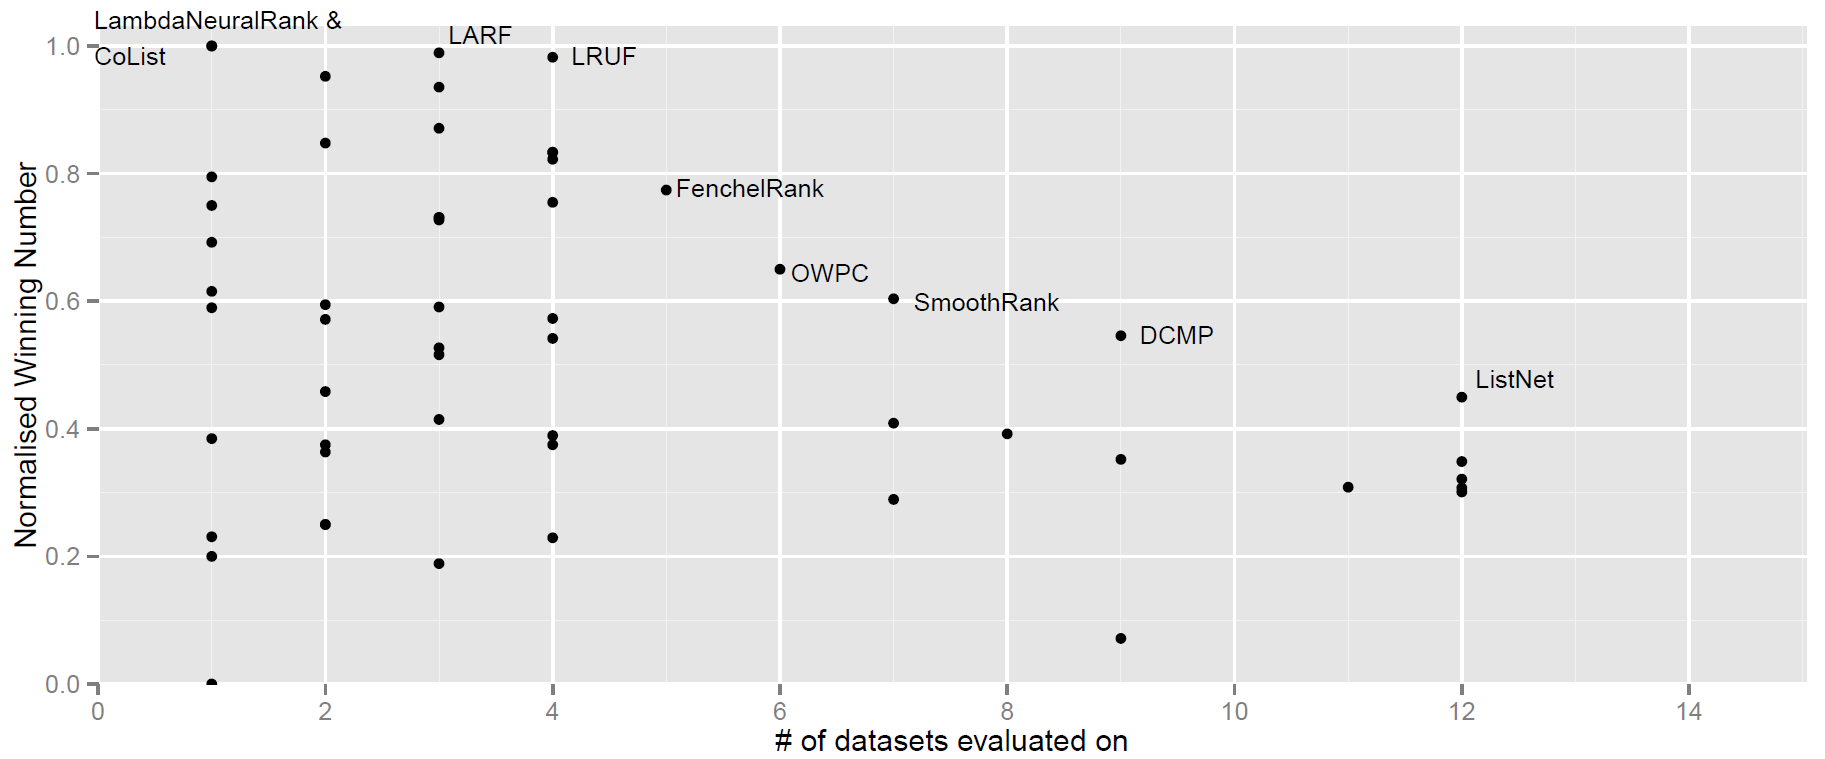
\includegraphics[scale=0.35]{gfx/ndcg3_winnum}
\caption{\acs{NDCG}@3 comparison of Learning to Rank methods}
\label{fig:normalised_winning_number_NDCG3}
\end{figure}

LambdaNeuralRank and CoList both acquired a perfect \ac{NWN} score of 1.0 by beating all other algorithms on one dataset, with LambdaNeuralRank winning on the AOL dataset and CoList winning on Yahoo! Set 2. LARF and LRUF both scored very high scores of near 1.0 on three of the LETOR 3.0 data sets, which can be said to have a higher degree of certainty on the methods' performance because they are validated on three data sets which in addition are more relevant data sets than AOL and Yahoo! Set 2 because there are more evaluation results available for the LETOR 3.0 data sets (see Table \ref{tab:ltr_methods_used}). FenchelRank, OWPC, SmoothRank, DCMP and ListNet are in that order increasingly lower in \ac{NWN}, but increasingly higher in number of data sets that they are evaluated on, resulting in a higher degree of certainty on the accuracy of the algorithms.\\

LambdaNeuralRank, CoList, LARF, LRUF, OWPC and DCMP evaluation results are all based on one study, therefore are subjected to the risk of one overly optimistic study producing those results. FenchelRank evaluation result are based combined result from two studies, although those studies have overlap in authors. SmoothRank and ListNet have the most reliable evaluation result source, as they were official LETOR baseline runs.  

\subsection{NDCG@5}
Figure \ref{fig:normalised_winning_number_NDCG5} shows the performance of Learning to Rank methods for the \ac{NDCG}@5 metric. Table \ref{tab:raw_data_norm_winnum_ndcg35} in Appendix \ref{app:norm_winnum_ndcg35} provides the raw Normalised Winning Number data for the Learning to Rank methods.\\

\begin{figure}[!h]
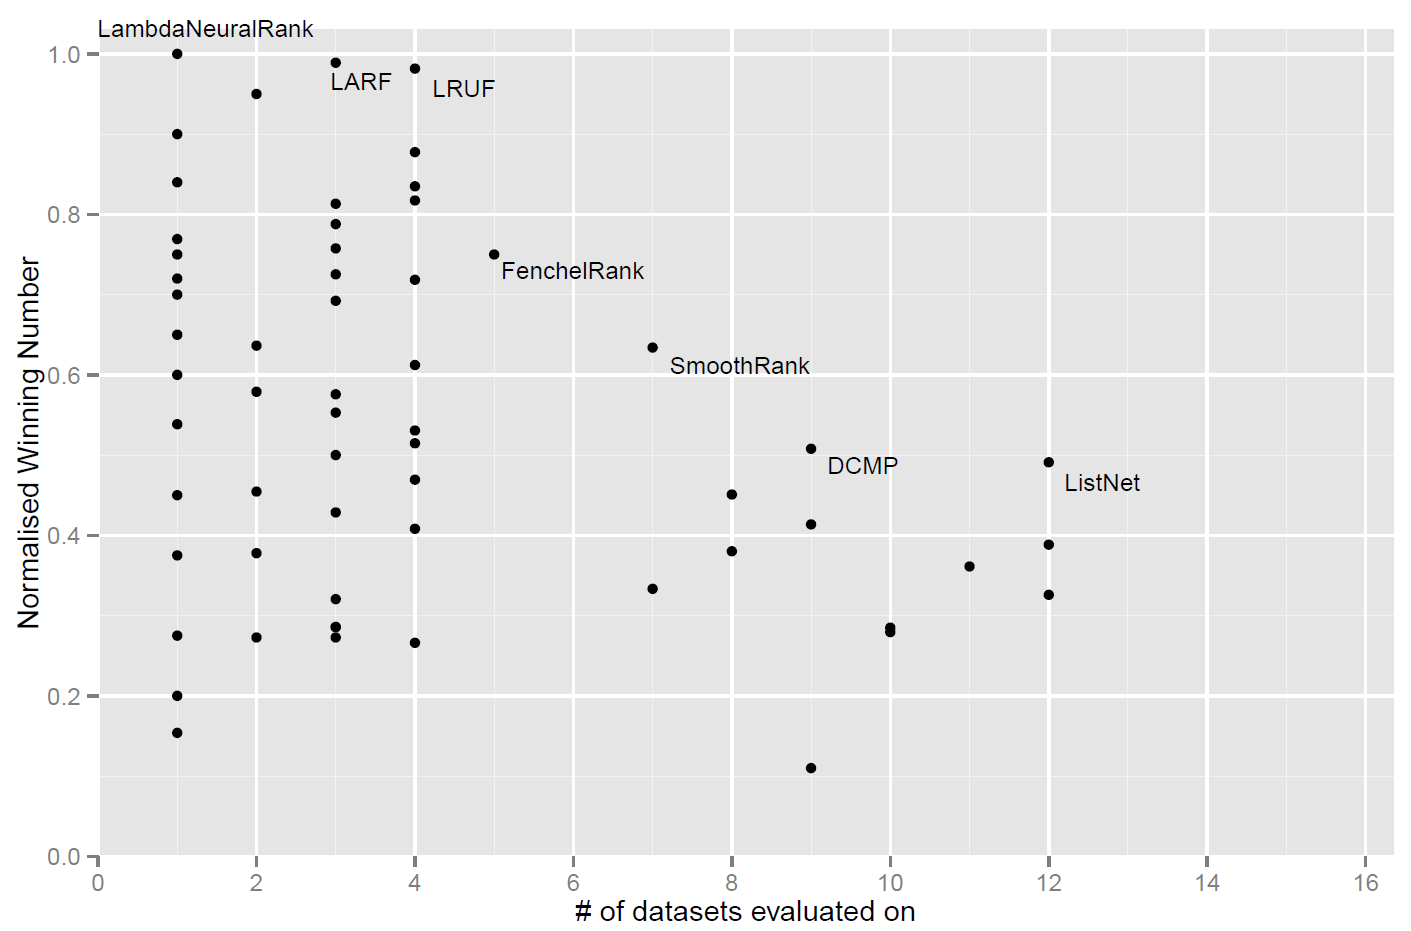
\includegraphics[scale=0.35]{gfx/ndcg5_winnum}
\caption{\acs{NDCG}@5 comparison of Learning to Rank methods}
\label{fig:normalised_winning_number_NDCG5}
\end{figure}

LambdaNeuralRank again beat all other methods solely with results on the AOL dataset scoring a \ac{NWN} of 1.0. LARF, LRUF, FenchelRank, SmoothRank, DCMP and ListNet are from left to right evaluated on an increasing number of data sets, but score decreasingly well in terms of \ac{NWN}. These results are highly in agreement with the \ac{NDCG}@3 comparison. The only modification compared to the \ac{NDCG}@3 comparison being that OWPC did show to be a method for which there were no methods performing better on both axes in the \ac{NDCG}@5 comparison, but not in the \ac{NDCG}@3 comparison. Like in the \ac{NDCG}@3 comparison, SmoothRank and ListNet can be regarded as most reliable results because the evaluation measurements for these methods are based on LETOR official baselines.

\subsection{NDCG@10}
Figure \ref{fig:normalised_winning_number_NDCG10} shows the performance of Learning to Rank methods for the \ac{NDCG}@10 metric. Table \ref{tab:raw_data_norm_winnum_ndcg10map} in Appendix \ref{app:norm_winnum_ndcg10map} provides the raw Normalised Winning Number data for the Learning to Rank methods.\\

\begin{figure}[!h]
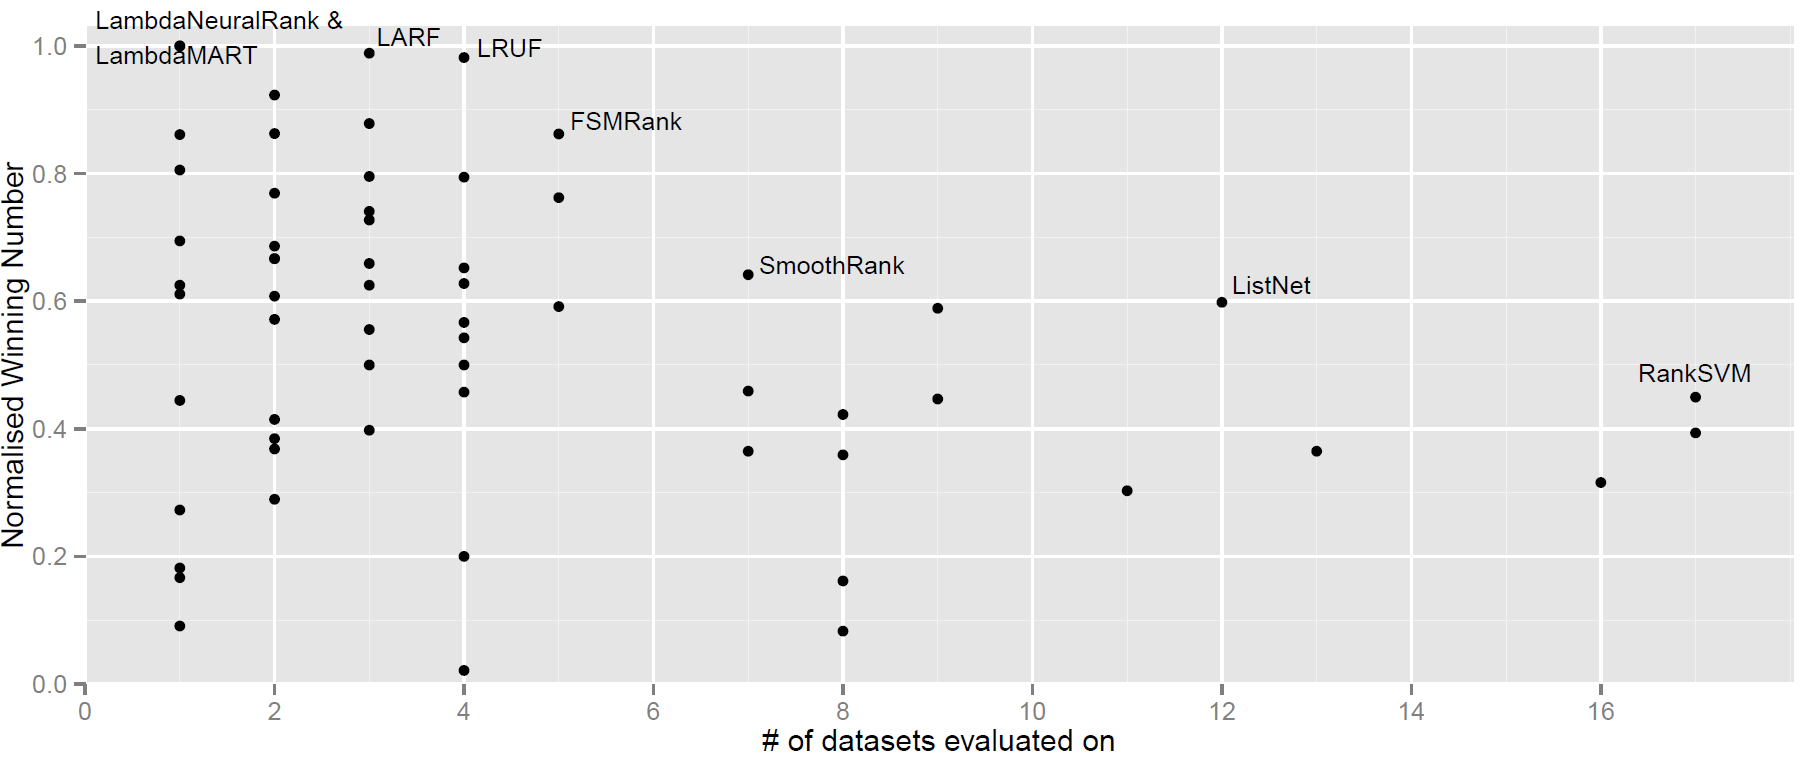
\includegraphics[scale=0.35]{gfx/ndcg10_winnum}
\caption{\acs{NDCG}@10 comparison of Learning to Rank methods}
\label{fig:normalised_winning_number_NDCG10}
\end{figure}

LambdaMART and LambdaNeuralRank score a \ac{NWN} of 1.0 on the \ac{NDCG}@10 comparison. For LambdaNeuralRank these results are again based on AOL dataset measurements. LambdaMART showed the highest \ac{NDCG}@10 performance for the MSLR-WEB10k dataset. The set of algorithms for which there is no other algorithm with both a higher \ac{NWN} and number of data sets evaluated on is partly in agreement with those for the \ac{NDCG}@3 and \ac{NDCG}@5 comparisons: {LARF, LRUF, FSMRank, SmoothRank, ListNet, RankSVM}. SmoothRank and FSMRank were not present in this set for the \ac{NDCG}@3 and \ac{NDCG}@5 comparison, but were close by, as can be seen in Tables \ref{tab:raw_data_norm_winnum_ndcg35} in Appendix \ref{app:norm_winnum_ndcg35}. DCMP is not in the set in contrast with the \ac{NDCG}@3 and \ac{NDCG}@5 comparison.

\subsection{MAP}
Figure \ref{fig:normalised_winning_number_map} shows the performance of Learning to Rank methods for the \ac{MAP} metric. Table \ref{tab:raw_data_norm_winnum_ndcg10map} in Appendix \ref{app:norm_winnum_ndcg10map} provides the raw \ac{NWN} data for the Learning to Rank methods.\\

\begin{figure}[!h]
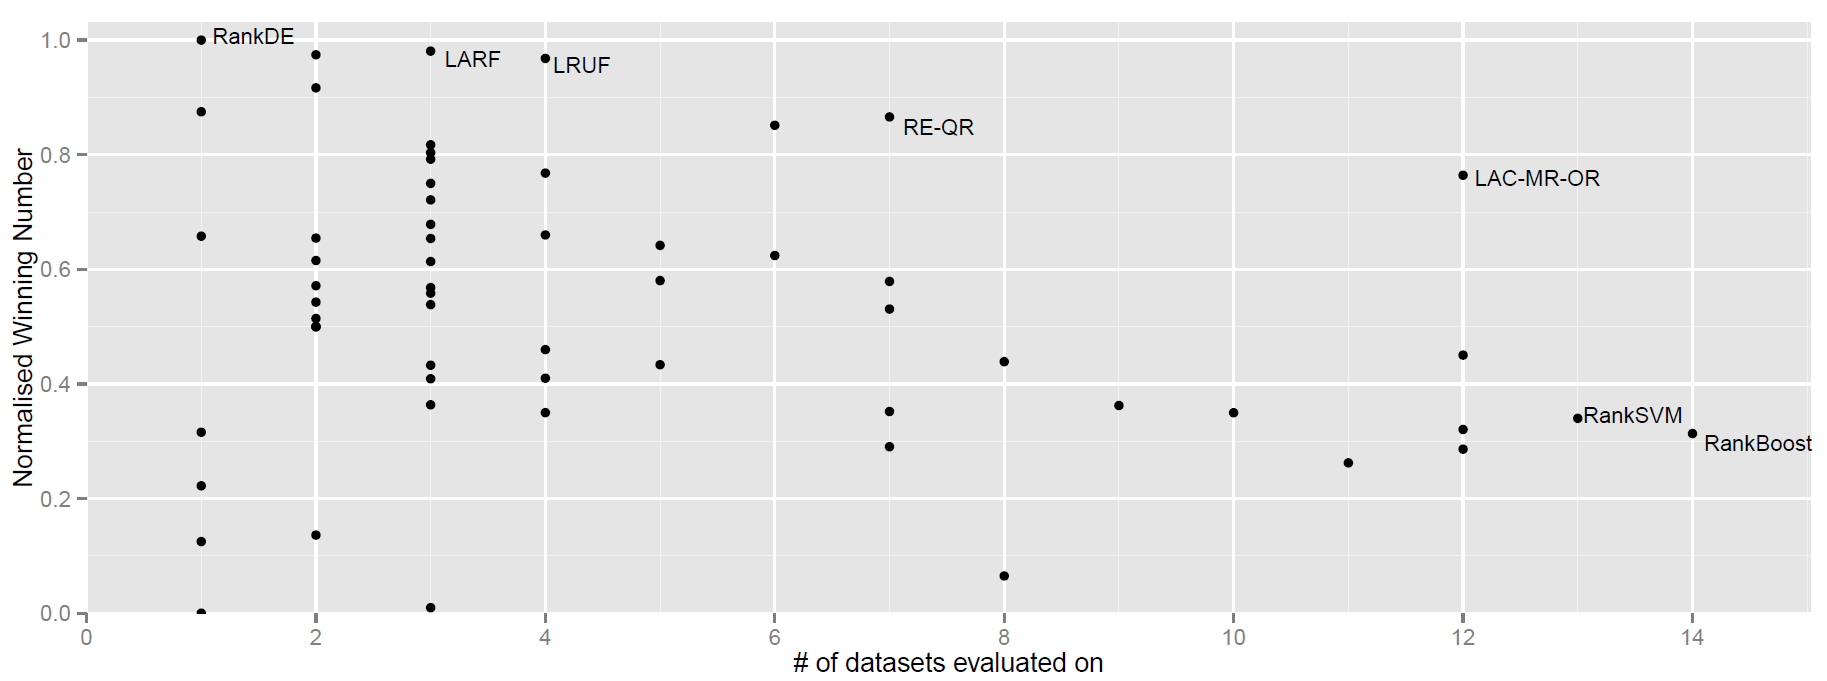
\includegraphics[scale=0.35]{gfx/map_winnum}
\caption{\acs{MAP} comparison of Learning to Rank methods}
\label{fig:normalised_winning_number_map}
\end{figure}

Where comparisons on the \ac{NDCG}-metric at different cut-off points where highly in agreement in terms of the best performing algorithms, the comparison in terms of \ac{MAP} shows different results. RankDE scores a \ac{NWN} of 1.0 on one dataset, like LambdaNeuralRank did on for all \ac{NDCG}-comparisons. In contrast to LambdaNeuralRank, RankDE achieved this highest score on the LETOR 2.0 TD2003, a dataset on which many methods are evaluated.\\

LARF and LRUF score very high \ac{NWN} scores, but based on only relatively few data sets, just as in the \ac{NDCG}-comparisons. Notable is that SmoothRank and ListNet, which showed both high accuracy and high certainty on all \ac{NDCG}-comparisons, are not within the best performing methods in the \ac{MAP}-comparison. A deeper look in the raw data Tables \ref{tab:raw_data_norm_winnum_ndcg35} and \ref{tab:raw_data_norm_winnum_ndcg10map} in Appendices \ref{app:norm_winnum_ndcg35} and \ref{app:norm_winnum_ndcg10map} respectively shows that LAC-MR-OR is evaluated on many more data sets for \ac{MAP} compared to \ac{NDCG}, which resulted in LAC-MR-OR obtaining equal certainty to ListNet with a higher \ac{NWN}. SmoothRank performed a \ac{NWN} of around 0.53 over 7 data sets, which is still good in both certainty and accuracy, but not among the top methods. RE-QR is one of the best performers in the \ac{MAP}-comparison with a reasonable amount of benchmark evaluations. No reported \ac{NDCG} performance was found in the literature study for RE-QR. There is a lot of certainty on the accuracy of RankBoost and Rank\acs{SVM} as both models are evaluated on the majority of data sets included in the comparison for the \ac{MAP}-metric, but given their \ac{NWN} it can said that both methods are not within the top performing Learning to Rank methods.

\subsection{Cross-metric}
Figure \ref{fig:normalised_winning_number_all} shows the \ac{NWN} as function of \ac{IWN} for the methods described in Table \ref{tab:ltr_methods_used}. Table \ref{tab:raw_data_norm_winnum_all} in Appendix \ref{app:norm_winnum_all} provide the raw data plotted in Figure \ref{fig:normalised_winning_number_all}.\\

\begin{figure}[!h]
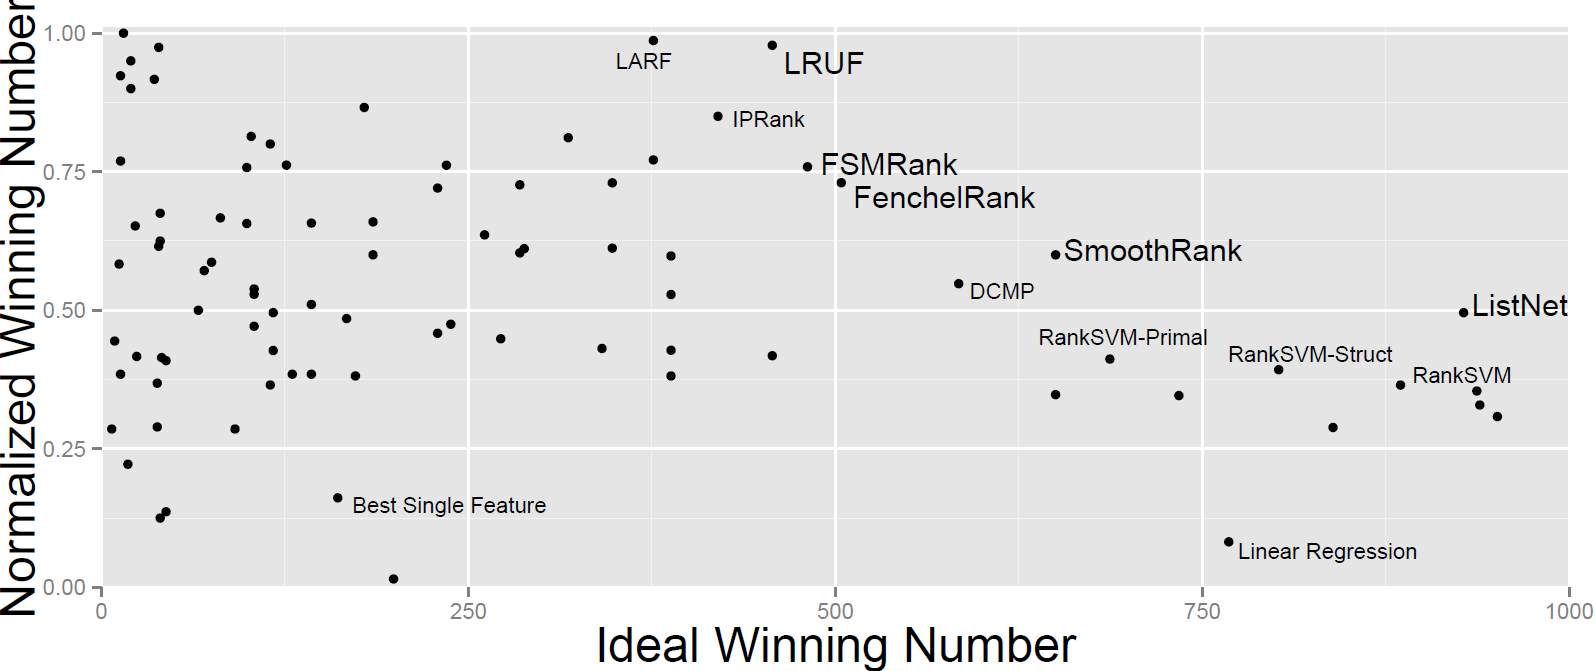
\includegraphics[scale=0.405]{gfx/combined_normalized_winnum}
\caption{Cross-benchmark comparison of Learning to Rank methods}
\label{fig:normalised_winning_number_all}
\end{figure}

The cross-metric comparison is based on the \ac{NDCG}@3, \ac{NDCG}@5, \ac{NDCG}@10 and \ac{MAP} comparisons combined, which justifies analysing the comparison more thoroughly. Figure \ref{fig:normalised_winning_number_all} labels the algorithms with no other algorithm having a higher value on both the horizontal axis and vertical axis, but also labels the algorithms with exactly one algorithm having a higher value on both axes with smaller font size. In addition, Linear Regression and the ranking method of simply sorting on the best single feature are labelled as baselines.\\

LRUF, FSMRank, FenchelRank, SmoothRank and ListNet showed to be the methods that have no other method superior to them in both \ac{IWN} and \ac{NWN}. LRUF is the only method that achieved this in all \ac{NDCG} comparisons, the \ac{MAP} comparison as well as the cross-metric comparison. With FenchelRank, FSMRank, SmoothRank and ListNet being among the top performing methods in all \ac{NDCG} comparisons as well as in the cross-metric comparison, it can be concluded that the cross-metric results are highly defined by the \ac{NDCG} performance as opposed to the \ac{MAP} performance. This was to be expected, because the cross-metric comparison input data of three \ac{NDCG} entries (@3, @5, and @10) enables it to have up to three times as many as many weight as the \ac{MAP} comparison.\\

LARF, \acs{IP}Rank and DCMP and several variants of Rank\ac{SVM} performed very well on the cross-metric comparison, with all having only one method in its top right quadrant. LARF also performed among the top methods on the \ac{NDCG} and \ac{MAP} comparisons and DCMP was a top performer in a few of the \ac{NDCG} comparisons.\\

C-CRF, DirectRank, FP-Rank, RankCSA, LambdaNeuralRank and VFLR all have near-perfect \ac{NWN} measures, but have low \ac{IWN} measures. Further evaluation runs of these methods on benchmark data sets that they are not yet evaluated on are desirable. The DirectRank paper \cite{Tan2013} shows that the method  is evaluated on more data sets than the number of data sets that we included evaluation results for in this meta-analysis. Some of the DirectRank measurements could not be used because measurements on some data sets were only available in graphical form and not in raw data.\\

LAC-MR-OR and RE-QR showed very good ranking accuracy in the \ac{MAP} comparison on multiple data sets. Because LAC-MR-OR is only evaluated on two data sets for \ac{NDCG}@10 and RE-QR is not evaluated for \ac{NDCG} at all, LAC-MR-OR and RE-QR are not within the top performing methods in the cross-metric comparison. 

\section{Limitations}
In the \ac{NWN} calculation the weight of each benchmark on the total score is determined by the number of evaluation measurements on this benchmark. By calculating it in this way, we implicitly make the assumption that the Learning to Rank methods are (approximately) distributed uniformly over the benchmarks, such that the average Learning to Rank method tested are approximately equally hard for each data set. It could be the case however that this assumption is false and that significantly more accurate Learning to Rank methods are evaluated on some data sets than on other data sets. \\

A second limitation is that the data sets on which Learning to Rank methods have been evaluated can not always be regarded a random choice. It might be the case that some researchers chose to publish results for exactly those benchmark data sets that showed the most positive results for their Learning to Rank method.\\

Another limitation is that our comparison methodology relies on the correctness of the evaluation results found in the literature search step. This brings up a risk of overly optimistic evaluation results affecting our \ac{NWN} results. Limiting the meta-analysis to those studies that report comparable results on one of the baseline methods of a benchmark set reduces this limitation but does not solve it completely. By taking \ac{IWN} into account in Figure \ref{fig:normalised_winning_number_all} we further mitigate this limitation, as \ac{IWN} is loosely related with the number of studies that reported evaluation results for an algorithm.\\

Our comparison regarded evaluation results on \ac{NDCG}@$\{3,5,10\}$ and \ac{MAP}. By making the decision to include \ac{NDCG} at three cut-off points and only a single \ac{MAP} entry, we implicitly attain a higher weight for \ac{NDCG} compared to \ac{MAP} on an analysis that combines all measurements on the four metrics. This implicit weighting could be regarded as arbitrary, but the number of algorithm evaluation results gained by this makes it a pragmatic approach. Note that another implicit weighting lies in the paper dimension. Hence, the higher number of evaluation results specified in a paper, the higher the influence of this paper on the outcome of the analysis. This implicit weighting is not harmful to the validity of our comparison, as papers with a large number of evaluation results are more valuable than papers with a few evaluation results. In addition, papers with a high number of evaluation results are not expected to be less reliable than papers with fewer evaluation results.

\section{Conclusions}
We proposed a new way of comparing learning to rank methods based on sparse evaluation results data on a set of benchmark datasets. Our comparison methodology comprises of two components: 1) \ac{NWN}, which provides insight in the ranking accuracy of the learning to rank method, and 2) \ac{IWN}, which gives insight in the degree of certainty concerning the performance of the ranking accuracy.\\

Based on this this new comparison approach for a set of sparse evaluation results, we will now look back on the first research question of the thesis.
\begin{description}
\item[RQ1] What are the best performing Learning to Rank algorithms in terms of ranking accuracy on relevant benchmark data sets?\\
\end{description}
Although no closing arguments can be formulated on which Learning to Rank methods are most accurate, a lot of insight has been gained with the cross-benchmark comparison on which methods tend to perform better than others.\\

Based on our literature search for evaluation results on well-known benchmarks collections, a lot of insight has been gained with the cross-benchmark comparison on which methods tend to perform better than others. However, no closing arguments can be formulated on which learning to rank methods are most accurate. LRUF, FSMRank, FenchelRank, SmoothRank and ListNet were the learning to rank algorithms for which it holds that no other algorithm produced more accurate rankings with a higher degree of certainty of ranking accuracy. From left to right, the ranking accuracy of these methods decreases while the certainty of the ranking accuracy increases.\\

LRUF, FSMRank, FenchelRank, SmoothRank and ListNet were the Learning to Rank algorithms for which it holds that no other algorithm produced more accurate rankings with a higher degree of certainty of ranking accuracy. From left to right, the ranking accuracy of these methods decreases while the certainty of the ranking accuracy increases. For more definite conclusions on the relative performance of these five methods, more evaluation runs on are desirable for the methods on the left side on the list on benchmark data sets that these methods have not yet been evaluated on.\\

More evaluation runs are needed for the methods on the left side of Figure \ref{fig:normalised_winning_number_all}. Our work contributes to this by identifying promising learning to rank methods that researchers could focus on in performing additional evaluation runs.\\

In the following chapters of this thesis, concerning parallel execution of the Learning to Rank training phase, the scope will be limited to the five methods that turned out to be superior Learning to Rank methods in terms of ranking accuracy and certainty about this ranking accuracy: LRUF, FSMRank, FenchelRank, SmoothRank and ListNet. Although it can not be concluded that these methods are inarguably the most accurate Learning to Rank methods, a strong presumption has been raised that these five Learning to Rank are accurate ranking methods.\\
\chapter{Selected Learning to Rank Methods}
\include*{Chapters/LTRMethods}
\chapter{Implementation}
\label{chap:implementation}
The first section of this chapter will briefly discuss the HDInsight platform, the Hadoop ecosystem components offered by HDInsight and, in this regard, the Hadoop components used for implementation of the algorithms described in Chapter \ref{chap:ltr_methods}. The second section of this chapter describes a Java framework that handles the joint components needed for MapReduce Learning to Rank computation that are independent of the Learning to Rank model. The subsequent sections describe the implementation details of specific Learning to Rank models.

\section{Architecture}
Ranking algorithms consist of a sequence of operations on the input data which are often, but not always, of iterative nature. Apache Pig \cite{Olston2008} will be used to implement the sequence of operation on the input data. Pig Latin, the data processing language that runs on Apache Pig, designed based on the observation that the traditional MapReduce paradigm is too low-level and rigid, and holds the middle between the declarative style of SQL and the procedural style of MapReduce. The Apache Pig system translates Pig Latin into MapReduce plans that are executed over Hadoop. The choice to implement the Learning to Rank algorithms in Pig Latin allow more focus on the data operations and less focus on low-level implementation details compared to native Hadoop MapReduce. Furthermore, it allows us to rely on Apache Pig to create efficient MapReduce plans out of the Pig Latin code which lowers the implementation-dependent factor of the experiments.\\

\subsection{Storing Input Data for HDInsight Processing}
Azure HDInsight supports both the traditional \ac{HDFS} as described by Shvacko et al. \cite{Shvachko2010}, as well as Microsoft's own \ac{WASB} storage solution. Blob storage decouples the storage from the HDInsight Hadoop cluster; it enables safe deletion of a HDInsight cluster without losing data, as data is not solely stored on the cluster itself, but also on a separate storage that is not cluster-dependent. Azure \ac{WASB} storage allows the user to select one of their data centre for storage. \ac{WASB} storage in the West Europe region (located in Amsterdam) will be used for storage, as this data centre is located close to where the experiments are executed.

\subsection{Microsoft Azure HDInsight Job submission}
Microsoft offers a scalable and on-demand Hadoop service with HDInsight, that enables Hadoop services for those not able to make the required investments for their own cluster. The latest HDInsight of HDInsight available at the time of writing, HDInsight 3.1, runs the Hortonworks distribution of Hadoop version 2.4. HDInsight 3.1 offers multiple ways of submitting Hadoop jobs to a HDInsight cluster, described in Table \ref{tbl:hdinsight_endpoints}.\\

\begin{table}
\centering
\begin{tabular}{p{4.2cm}p{2.6cm}p{5.5cm}}\toprule
Job submission method & Type & Description \\
\midrule
Powershell & Powershell scripts & The Azure module for Windows PowerShell enables direct submission of Hadoop jobs through PowerShell cmdlets.\\
C\# API & C\# API & A wrapper API is offered to submit Hadoop MapReduce jobs directly from C\# code.\\
HiveServer/HiveServer2 & REST endpoint & Apache Hive \cite{Thusoo2009} is an open-source data warehousing solution on top of Hadoop, that supports processing of a SQL-like declarative language called HiveQL. HiveServer and its successor HiveServer 2 are REST endpoints that allow remote submission of HiveQL queries.\\
Oozie & REST endpoint & Apache Oozie \cite{Islam2012} is a workflow scheduler to manage Apache Hadoop jobs. Oozie enables users to specify Directed Acyclical Graphs of action, where each action is specified in either MapReduce or Pig.\\
WebHCat/Templeton & REST endpoint & WebHCat, formerly known as Templeton, is a REST API for HCatalog, a table and storage management layer for Hadoop. WebHCat allows users to use either Apache Pig, Apache MapReduce or Apache Hive for data processing.\\	
\bottomrule
\end{tabular}
\caption{HDInsight REST endpoints for job submission}
\label{tbl:hdinsight_endpoints}
\end{table}

Oozie and WebHCat/Templeton are the two methods for job submission in Table \ref{tbl:hdinsight_endpoints} that both 1) support Apache Pig jobs, and 2) Can be used from within Java code. Below the necessary procedures for job submission from Oozie as well as from WebHCat will be sketched.\\

% TODO: Stuk over werkzaamheden framework uitbreiden: uitlezen resultaten (evaluatieresultaten + doorgeven tussenresultaten (die tweede wellicht later in het document pas introduceren))
Fold handling  in a cross-validation experiment is the process of loading the correct data folds for training, validation and testing in the multiple rounds that the cross-validation experiment consists of. Fold handling is a task that needs to be taken care of regardless of the ranking model that is being evaluated. Given that most ranking models are of an iterative nature, the task of iteration handling is also a task that need to be done for most models. Iteration handling and fold handling are procedures in which the same steps are repeated for each iteration or cross-validation round respectively. Pig Latin, however, has no support for loops which are needed to perform iteration handling and fold handling. Since iteration handling and fold handling are tasks that need to be addressed for each ranking model and that cannot be solved with Pig, we create a framework that takes care of both iteration and fold handling and generates the Pig Latin code for the current iteration and fold. The aim of this framework is to let implementations of ranking models focus solely on implementing the sequential steps of one iteration of the algorithm, while the framework arranges that 1) these sequential steps are performed iteratively and 2) these sequential steps are performed on the multiple training folds of data. This framework that handles folding and iterations will be implemented in Java and will work such that fold- and iteration dependent parts of the Pig code will be generated dynamically by the Java framework after which the Pig job will be sent to the cluster.\\

Another responsibility of the framework is to handle communication between multiple Pig jobs within a single iteration of a Learning to Rank algorithm. The framework enables reading the result of a Pig job from \ac{WASB} storage which can then be used as parameter within a subsequent Pig job. An example of this is a Pig implementation of gradient descent, where a first Pig job might calculate gradients and writes them to storage, after which the framework assists in reading the gradients from storage and allows them to be used as input parameters of a second Pig job that calculates new feature weights based on its gradient parameter and a predetermined step size.\\

\begin{table}
\centering
\begin{tabular}{p{5cm}p{5cm}}\toprule
Job submission procedure for Apache Oozie & Job submission procedure for WebHCat/Templeton \\
\midrule
1. Let the framework build the Pig job dynamically. & 1. Let the framework build the Pig job dynamically.\\
2. Encapsulate the Pig job in an Oozie workflow. & 2. Submit the Pig job through the WebHCat/Templeton REST API.\\
3. Upload the Oozie workflow to HDFS storage. & \\
4. Execute the Oozie workflow through the Oozie REST API. & \\
\bottomrule
\end{tabular}
\caption{Comparison of Oozie and WebHCat job submission procedures}
\label{tbl:oozie_templeton}
\end{table}

Table \ref{tbl:oozie_templeton} shows how Oozie job submission is more complex then for the case of dynamically generated jobs than WebHCat/Templeton. Oozie is more fitting for static Hadoop jobs that require a workflow consisting of a sequence of Pig and MapReduce jobs mixed together, but is a lesser fit for our situation. Templeton will be used for submission of the Pig jobs, as the HDInsight version that was available at the start of the implementation did not yet support WebHCat.

\subsection{ListNet}
The following sections describe the Pig jobs that form the three independent parts of the ListNet ranking model: 1) Preprocessing, 2) Training (this includes evaluation over the validation set) and 3) Testing (evaluation over the test set). 
\subsubsection{Preprocessing}
The preprocessing phase consists of two separate Pig jobs. The first Pig job determines the minimum and the maximum values per feature in the training set. The second Pig job rescales each feature of the train, validation and test datasets using the following formula for rescaling:
\begin{equation}
x^{'} = \frac{x-min(x)}{max(x)-min(x)}
\end{equation}
This rescaling procedure sets the values of all features to be within range $[0,1]$.\\

The first Pig job:\\
\begin{minipage}{\linewidth}
\begin{lstlisting}
REGISTER [path prefix]/lib/*.jar;
TRAIN = LOAD '[path prefix]/input/[dataset name]/Fold[fold number]/train.txt' USING PigStorage(' ');
TRAIN_STD = FOREACH TRAIN GENERATE flatten(udf.util.ToStandardForm(*));
TRAIN_STD_BY_QUERY = GROUP TRAIN_STD BY $1 PARALLEL [available reducers];
MIN_MAX = FOREACH TRAIN_STD_BY_QUERY GENERATE flatten(udf.util.GetMinMax(*));
MIN_MAX_GRPD = GROUP MIN_MAX ALL;
MIN_MAX_FIN = FOREACH MIN_MAX_GRPD GENERATE flatten(udf.util.CombineMinMax(*));
STORE MIN_MAX_FIN INTO 'minmax[fold number]';
\end{lstlisting}
\end{minipage}

The minimum and maximum values per feature stored in MIN\_MAX\_FIN can now be read from \ac{HDFS} and used within the Java framework by using the Windows Azure Storage library. The second Pig job uses these minimum and maximum values by parametrising the \ac{UDF} that performs the rescaling transformation, udf.util.ScaleFeatures(), with the minimum and maximum feature values.\\

\begin{table}
\centering
\begin{tabular}{p{5cm}p{8cm}}\toprule
UDF & Description \\
\midrule
udf.util.ToStandardForm() & Transforms the data set into the standard form of relevance label in first column followed by feature values. Strips data of any other columns, if present.\\
udf.util.GetMinMax() & Extracts the minimum and maximum value per feature, for the documents of a single query.\\
udf.util.CombineMinMax() & Combines outputs of the udf.util.GetMinMax() UDF for each query into globally minimum and maximum feature values.\\
\bottomrule
\end{tabular}
\caption{Description of preprocessing User Defined Functions (1/2)}
\label{tbl:preprocessing_udfs_1}
\end{table}

The second Pig job:\\
\begin{minipage}{\linewidth}
\begin{lstlisting}
REGISTER [path prefix]/lib/*.jar;
TRAIN = LOAD '[path prefix]/input/[dataset name]/Fold[fold number]/train.txt' USING PigStorage(' ');
VALIDATE = LOAD '[path prefix]/input/[dataset name]/Fold[fold number]/vali.txt' USING PigStorage(' ');
TEST = LOAD '[path prefix]/input/[dataset name]/Fold[fold number]/test.txt' USING PigStorage(' ');
TRAIN_STD = FOREACH TRAIN GENERATE flatten(udf.util.ToStandardForm(*));
VALIDATE_STD = FOREACH VALIDATE GENERATE flatten(udf.util.ToStandardForm(*));
TEST_STD = FOREACH TEST GENERATE flatten(udf.util.ToStandardForm(*));
DEFINE ScaleFeatures udf.util.ScaleFeatures('[array with minimum and maximum feature values]');
TRAIN_SCA = FOREACH TRAIN_STD GENERATE flatten(ScaleFeatures(*));
VALIDATE_SCA = FOREACH VALIDATE_STD GENERATE flatten(ScaleFeatures(*));
TEST_SCA = FOREACH TEST_STD GENERATE flatten(ScaleFeatures(*));
STORE TRAIN_SCA INTO 'train_sca[fold number]' USING BinStorage();
STORE VALIDATE_SCA INTO 'validate_sca[fold number]' USING BinStorage();
STORE TEST_SCA INTO 'test_sca[fold number]' USING BinStorage();
\end{lstlisting}
\end{minipage}

\begin{table}
\centering
\begin{tabular}{p{5cm}p{8cm}}\toprule
UDF & Description \\
\midrule
udf.util.ToStandardForm() & See Table \ref{tbl:preprocessing_udfs_1} for description.\\
udf.util.ScaleFeatures() & Uses the minimum and maximum feature values with which it is parametrised perform the following rescaling transformation to the features: $x^{'} = \frac{x-min(x)}{max(x)-min(x)}$.\\
\bottomrule
\end{tabular}
\caption{Description of preprocessing User Defined Functions (2/2)}
\label{tbl:preprocessing_udfs_2}
\end{table}

\subsubsection{Training}
The training stage, like the preprocessing stage, consists of two separate Pig jobs. The first Pig job calculates the Cross Entropy loss on training data of the current model and calculates the gradients for the next model update. The second Pig job is an internal validation step that validates the model on the validation set by calculating \ac{nDCG}@k.\\

The first Pig job:\\
\begin{minipage}{\linewidth}
\begin{lstlisting}
REGISTER [path prefix]/lib/*.jar;
DEFINE QueryLossGradient udf.listnet.QueryLossGradient('[feature dimensionality of data set]');
DEFINE ExpRelOurScores udf.listnet.ExpRelOurScores('[neural network weights & iteration number]');
[FIRST TRAINING ITERATION:]
	TRAIN_SCA = LOAD 'train_sca[fold number]/*' USING BinStorage();
	TR_BY_QUERY = GROUP TRAIN_SCA BY $1 PARALLEL [number of avaiable reducers];
	TR_EXP_REL_SCORES = FOREACH TR_BY_QUERY GENERATE flatten(ExpRelOurScores(TRAIN_SCA));
	STORE TR_EXP_REL_SCORES INTO 'tr_exp_rel_scores-f[fold number]' USING BinStorage();
[SUBSEQUENT TRAINING ITERATIONS:]
	TR_EXP_REL_SCORES = LOAD 'tr_exp_rel_scores-f[fold number]/*' USING BinStorage();
	TR_EXP_REL_SCORES = FOREACH TR_EXP_REL_SCORES GENERATE flatten(ExpRelOurScores(*)) PARALLEL [number of available reducers];
TR_QUERY_LOSS_GRADIENT = FOREACH TR_EXP_REL_SCORES GENERATE flatten(QueryLossGradient(*)) PARALLEL [number of available reducers];
TR_QUERY_LOSS_GRADIENT_GRPD = GROUP TR_QUERY_LOSS_GRADIENT ALL;
TR_LOSS_GRADIENT = FOREACH TR_QUERY_LOSS_GRADIENT_GRPD GENERATE flatten(udf.listnet.MultiSum(*));
STORE TR_LOSS_GRADIENT INTO 'tr_loss_gradient-f[fold number]i[iteration number]';
\end{lstlisting}
\end{minipage}

\begin{table}
\centering
\begin{tabular}{p{5cm}p{8cm}}\toprule
UDF & Description \\
\midrule
udf.listnet.QueryLossGradient() & Calculates the Cross Entropy loss for a query and calculates the gradients per feature based on this query.\\
udf.listnet.ExpRelOurScores() & Calculates the predicted relevance label of a query based on the current model weights and transforms this following the transformation $x -> e^{x}$. In case the current iteration is the first iteration, the same transformation is applied to the ground truth relevance label.\\
udf.listnet.MultiSum() & Calculates aggregated loss and feature gradients by summing the per-query losses and per-query feature gradients.\\
\bottomrule
\end{tabular}
\caption{Description of training User Defined Functions (1/2)}
\label{tbl:training_udfs_1}
\end{table}

The second Pig job of the training stage validates the performance of the model weights that were trained in the first Pig job on the validation data set.\\

The second Pig job:\\
\begin{minipage}{\linewidth}
\begin{lstlisting}
REGISTER [path prefix]/lib/*.jar;
DEFINE Ndcg udf.util.Ndcg('[neural network weights & NDCG cut-off parameter]');
[FIRST TRAINING ITERATION:]
	VALIDATE_SCA = LOAD 'validate_sca[fold number]/*' USING BinStorage();
	VA_BY_QUERY = GROUP VALIDATE_SCA BY $1 PARALLEL [number of available reducers];
	STORE VA_BY_QUERY INTO 'va_by_query-f[fold number]' USING BinStorage();
[SUBSEQUENT TRAINING ITERATIONS:]
	VA_BY_QUERY = LOAD 'va_by_query-f[fold number]/*' USING BinStorage();
NDCG = FOREACH VA_BY_QUERY GENERATE Ndcg(*);
NDCG_GRPD = GROUP NDCG ALL;
AVG_NDCG = FOREACH NDCG_GRPD GENERATE AVG(NDCG);
STORE AVG_NDCG INTO 'avg_ndcg-f[fold number]i[iteration number]';
\end{lstlisting}
\end{minipage}

\begin{table}
\centering
\begin{tabular}{p{5cm}p{8cm}}\toprule
UDF & Description \\
\midrule
udf.util.Ndcg() & Calculates \ac{nDCG}@k for a query.\\
\bottomrule
\end{tabular}
\caption{Description of training User Defined Functions (2/2)}
\label{tbl:training_udfs_2}
\end{table}

\subsubsection{Testing}
The testing stage tests the best model found in the training iterations, selected on validation set \ac{nDCG}@k (as calculated in the second Pig job of the training stage), by calculating the \ac{nDCG}@k of this model on the test set.\\

Test stage Pig job:\\
\begin{minipage}{\linewidth}
\begin{lstlisting}
REGISTER [path prefix]/lib/*.jar;
TEST_SCA = LOAD 'test_sca[fold number]/*' USING BinStorage();
TE_BY_QUERY = GROUP TEST_SCA BY $1 PARALLEL [number of available reducers];
DEFINE Ndcg udf.util.Ndcg('[neural network weights & NDCG cut-off parameter]');
NDCG = FOREACH TE_BY_QUERY GENERATE Ndcg(*);
NDCG_GRPD = GROUP NDCG ALL;
AVG_NDCG = FOREACH NDCG_GRPD GENERATE AVG(NDCG);
STORE AVG_NDCG INTO 'avg_ndcg';
\end{lstlisting}
\end{minipage}

\subsection{SmoothRank}
\chapter{MapReduce Experiments}
\include*{Chapters/Results}
\chapter{Conclusions}
\include*{Chapters/Conclusions}
\chapter{Future Work}
\section{Computing models}
We explored the possibilities of Hadoop MapReduce for computation

\section{Learning to Rank algorithms}
% ********************************************************************
% Backmatter
%*******************************************************
\cleardoublepage
\appendix
\include*{Chapters/AppendixA}
\include*{Chapters/AppendixB}
\include*{Chapters/AppendixC}
\include*{Chapters/AppendixD}
\include*{Chapters/AppendixE}
\include*{Chapters/AppendixF}
%********************************************************************
% Other Stuff in the Back
%*******************************************************
%********************************************************************
% Bibliography
%*******************************************************
% work-around to have small caps also here in the headline
\manualmark
\markboth{\spacedlowsmallcaps{\bibname}}{\spacedlowsmallcaps{\bibname}} % work-around to have small caps also
%\phantomsection 
\refstepcounter{dummy}
\addtocontents{toc}{\protect\vspace{\beforebibskip}} % to have the bib a bit from the rest in the toc
\addcontentsline{toc}{chapter}{\tocEntry{\bibname}}
\bibliographystyle{plainnat}
\label{app:bibliography} 
\bibliography{Bibliography}
% ********************************************************************
% Game Over: Restore, Restart, or Quit?
%*******************************************************
\end{document}
% ********************************************************************
